\documentclass[12pt]{report}
\usepackage[paper=a4paper,margin=2.7cm]{geometry}
\usepackage[utf8]{inputenc}
\usepackage{csquotes}
\usepackage{nameref}
\usepackage{graphicx}
\usepackage{amsmath}
\usepackage{textcomp}
\usepackage{eurosym}
\usepackage{float}
\usepackage{titlesec}
\usepackage{csvsimple}
\usepackage{lmodern}
\usepackage{wrapfig}
\usepackage{lipsum}
\usepackage{listings}
\usepackage{xcolor}
\usepackage{brufaceStyle}
\usepackage{setspace}
\onehalfspacing

\PassOptionsToPackage{hyphens}{url}\usepackage{hyperref}

\setlength\intextsep{0pt}


\colorlet{punct}{red!60!black}
\definecolor{background}{HTML}{EEEEEE}
\definecolor{delim}{RGB}{20,105,176}
\colorlet{numb}{magenta!60!black}

\lstdefinelanguage{json}{
    basicstyle=\normalfont\ttfamily,
    numbers=left,
    numberstyle=\scriptsize,
    stepnumber=1,
    numbersep=8pt,
    showstringspaces=false,
    breaklines=true,
    frame=lines,
    backgroundcolor=\color{background},
    literate=
     *{0}{{{\color{numb}0}}}{1}
      {1}{{{\color{numb}1}}}{1}
      {2}{{{\color{numb}2}}}{1}
      {3}{{{\color{numb}3}}}{1}
      {4}{{{\color{numb}4}}}{1}
      {5}{{{\color{numb}5}}}{1}
      {6}{{{\color{numb}6}}}{1}
      {7}{{{\color{numb}7}}}{1}
      {8}{{{\color{numb}8}}}{1}
      {9}{{{\color{numb}9}}}{1}
      {:}{{{\color{punct}{:}}}}{1}
      {,}{{{\color{punct}{,}}}}{1}
      {\{}{{{\color{delim}{\{}}}}{1}
      {\}}{{{\color{delim}{\}}}}}{1}
      {[}{{{\color{delim}{[}}}}{1}
      {]}{{{\color{delim}{]}}}}{1},
}

\usepackage[sorting=none]{biblatex}
\addbibresource{references.bib}

%\newcommand{\sectionbreak}{\clearpage}
\renewcommand{\contentsname}{Table of Contents}
\newlength\longest

\edef\restoreparindent{\parindent=\the\parindent\relax}
\usepackage{parskip}
\restoreparindent

\title{Master Thesis}
\subtitle{Computational simulation of an economical system: an empirical analysis of some key parameters}
\author{Ricardo Gomes Rodrigues\\000443812}
\academicYear{2020 - 2021}
\promotor{Promoter: Prof. Hugues Bersini}
\masterAndMajor{Master of Computer Science}{Major in Artificial Intelligence \& Optimization}


\begin{document}

\maketitle
\newpage

\chapter*{Abstract}



Through the use of computer simulations, we will try to better understand the role of a State and how its choices can impact its economy and agents. A State can implement many rules in order to achieve whatever goal it desires such as equity or efficiency. We will experiment and analyze many parameters that are present in our society and see how each parameter influences some important metrics. Finally, we will try to optimize some metrics through the use of Particle Swarm Optimization (PSO), a heuristic optimization algorithm.




\chapter*{Acknowledgements}
After 5 years at University, I have eventually come to this moment of writing my master thesis. I am insanely proud to have made it up until this moment to thank my family as well as my friends who have supported during all these years. 
I would especially like to thank my parents, Maria and Joaquim, who have unconditionally supported me (despite not understanding anything regarding what I was \emph{exactly} studying, they are not very tech-savvy).

I must also mention my fellow comrades Alexandre, Simon and Nicolas with whom I have spent hours, days, and even weeks working relentlessly on projects, assignments, exams, etc. We have known each other since the first year, and have always motivated one another to reach this final year of our degree, \emph{together}. I thank them deeply for all their supported as friends. I am thrilled to finish this year with them and also very proud of them.

I would also like to thank all of my Professors who have taught me so many things, some that I found incredibly interesting, some a bit less however, in the end, it was all necessary. I especially want to thank my promoter Prof. Hugues Bersini, who I had the chance to have as a Professor \emph{twice}, for his insights and the liberty he allowed me to have to do this thesis.

\clearpage

\thispagestyle{empty}

\vspace*{\fill}
\begin{center}
    ``I'm afraid that the following syllogism may be used by some in the future.
    
    Turing believes machines think\\
    Turing lies with men\\
    Therefore machines do not think
    
    Yours in distress,
    
    Alan.''
\end{center}

\begin{flushright}
    - Alan Turing
\end{flushright}


\vspace*{3cm}

\begin{center}
    ``Don't you ever let a soul in the world tell you that you can't be exactly who you are.''
\end{center}


\begin{flushright}
    - Lady Gaga
\end{flushright}


\vfill

\clearpage

\tableofcontents
\newpage

\chapter{Introduction}

\section{Introduction}

An economic system is a very complex set of mechanisms and rules in order to produce, exchange and consume goods and services. Despite its complexity, this structure is a key part of our day-to-day life and we will try to understand different parameters of our system and their influences on key aspects such as efficiency or equality.

Unfortunately, such systems are virtually impossible to pin down analytically due to the many roles, rules and parameters: no set of mathematical formulas can model them properly due because of many reasons such as the randomness introduced in the simulation, the large amounts of entities it is made of, the many parameters, etc.
As stated by Leigh Tesfatsion, numerous algorithms have already tried to model social processes. We can cite a few of them such as genetic algorithms or reinforcement learning algorithms (Q-learning for instance). These algorithms have been developed with one purpose: optimality \cite{tesfatsion_bottom_up}. 

In our case, we will use a computer-based simulation approach to study different types of economic systems. This approach will allow us to simulate a macro-structure (i.e. economic system) by the interactions of multiple autonomous micro-structures (i.e. agents) under a predefined set of rules. This approach falls into the area of Agent-based Computational Economics (ACE). The focus will put on the role of a State. More specifically, its redistributing role in order to correct the inequalities that may, and most probably will, occur in the system. 

It goes without saying that such a simulation cannot model perfectly an economic system either, however it lets us see emerging patterns that can be studied and analysed to better understand how and why our systems work or do not work. The definition of a working system is not universal, but in our case we will settle for a definition based on the efficiency and the equality of our system.

This trade-off has previously been studied by multiple people, in particular in the paper wrote by Hugues Bersini and Nicolas van Zeebroeck titled \textquote{Why should an economy be competitive?} \cite{bersini}. It draws the conclusion that a \textquote{competitive market is efficiently superior to a random market, however, inequalities will be much more present}. This thesis goes even further by incorporating the notion of a State whose main role will be to redistribute the money it collects from taxes for instance. 

The aforementioned paper applied an ACE-based approach to \textquote{simulate the interactions of agents producing and trading goods within different market structures}. As previously stated, the agent-based method works well in case of a bottom-up approach: the agents, that can  produce, consume and exchange, will interact with one another. With large amounts of autonomous agents, we will be able to study emerging phenomena and see how the rules and parameters influence our economical system. In order to do this, many key parameters have been incorporated into the simulation to make it as exhaustive as possible. All of these parameters (i.e. VAT rate, unemployment rate, etc.) can be tuned, analyzed (and optimized) to see the effects on key metrics such as the Gini coefficient or the number of transactions among others. 

Our simulation will be made of different models all working together - similarly to a society. These four main entities are: the State, the Agent, the Product and the Market. Each one contains essential parameters as well as multiple properties that will be studied as key metrics to understand the role of each parameter. We will precisely describe these models later on.


\section{Motivation and objectives}\label{section:motivation_objectives}

The motivation of this work comes from my curiousness in understanding the World that surrounds us. Mixing social sciences with computer sciences is a very interesting way to give us some keys to better understand \emph{why} our economical systems is the way it is through a simulation. It would also be interesting to see what could be done to make the system better: either to make it more efficient or more equal.

\subsection{Objectives}

This work will have many objectives and a wide range of questions will be studied. Because our models will have many parameters, it will be very interesting to study their influence on the system. We have three main objectives which are an empirical understanding of the system, a theory generation of the system \cite{tesfatsion_handbook} and eventually the optimization of the parameters.

In the first objective, the goal is to understand why some systems as we know them today have persisted. We will see which systems are viable and will not crash and see if it corresponds to the economic systems that we already know.

In the second objective, the purpose it to understand the impact of parameters and see how the system changes under different initial conditions. The dynamics of the system might change heavily with some parameters, less so with others.

Finally, an interesting goal would be to optimise all the parameters that we have mentioned so far. Because the searching space of these numerous parameters is vast, we plan on using another algorithm to tweak these parameters in order to reach two different goals which are at the antithesis from one another: the amount of money present in the system and its distribution among the agents. 

\subsection{Research questions}

The main research question that will be studied in this report is:

\vspace*{0.5cm}

\begin{center}
    How will the trade-off between efficiency and equality be affected by the parameters and choices we make when initializing our system?
\end{center}

\vspace*{0.5cm}

This question will depend on multiple factors that have already been studied in a real systems as we are going to see in the \nameref{section:state_of_the_art} chapter~\ref{section:state_of_the_art}. We will divide them into different categories representing the four models we have mentioned: the Product, the Agent, the State and the Market. 

\subsubsection{Products}

\begin{itemize}
    \item How does the selling price of a product affect its sales ?
    \item An agent can choose a product to buy from a variety of products available on the market. There are multiple strategies to pick a product, how will it affect the sales of a product for instance?
\end{itemize}


\subsubsection{Agents}

\begin{itemize}
    \item How will the money that an agent receives at the beginning affect its ability to purchase products ? What if, instead of all agents starting with the same amount of money, we make some agents richer and poorer than others? This is useful to study the equality of opportunity.
    \item What would happen if some agents do not pay their taxes (i.e. black or shadow economy) ? Would do State crash if an important part of its agents do not pay them? 
    \item What would happen if some agents never produce anything (i.e. unemployment) ?
    \item How can a non-producer agent make purchases ?
    \item How important are the skills that an agent has? 
\end{itemize}

\subsubsection{States}

\begin{itemize}
    \item How will the VAT value affect the EET? Extreme cases might be useful to study to see clearer patterns such as what would happen if the State collects 100\% of VAT? What about 0\%?
    \item What about the customs tax?
    \item What about the levy rate?
    \item How would a wealth tax affect the EET?
    \item Which redistribution system works the best?
    \item What if there is no redistribution system?
    \item Following the previous question, how important are the inequalities in such systems? What about the Gini coefficient? 
    \item How many connections does the State have? How does it affect the EET?
    \item How good (or bad) are the protectionism and the free trade policies?
    \item What is the importance of clusters? Do States that belong to a cluster perform better?
\end{itemize}

\subsubsection{Market}

\begin{itemize}
    \item How is the money distributed in the system ? 
\end{itemize}



\noindent We will also experiment the interactions of these entities. Finally, we can see that most of the questions we will try to answer revolve around the State's choices and how it impacts its agents with regards to the efficiency and equality. This is the main focus of this thesis.

\section{Notions and vocabulary}
To better understand the next parts of this thesis, we will briefly define a few terms which will frequently appear. Some of these will be thoroughly explained later when needed.

\begin{itemize}
    \item \textbf{ABM} Agent-Based Modelling (ABM) is a model used in computer simulations to simulate the actions and interactions between independent agents in the hope to see some patterns emerge.
    \item \textbf{GDP} The Gross Domestic Product is an economic tool which measures the wealth production of a country for a certain period. It is a key metric for the analyze of the health of a State.
    \item \textbf{Gini coefficient} The Gini coefficient is another economic metric which measures the wealth distribution among some agents (in a country for instance). It is a value between 0 and 1, where 0 means a perfectly equal society, whereas 1 represents a totally unequal society where one agent detains all the wealth.
\end{itemize}

\chapter{State of the Art}\label{section:state_of_the_art}

We will now depict the current state-of-the-art of what research is happening on the same topic in both economics and computer science.
Our goal will be to see if the state-of-the-art research presented hereunder does match the results that our simulation will yield. The state-of-the-art will not detail every metric thoroughly as the goal is to have an overview of these metrics and their roles, and not to do a thesis for each of them. Hence, we will briefly define the notion, see its application in the real world and analyze the importance of the parameter on other metrics according to the literature.

\section{In economics}

Prof. Bayenet, Professor of ``Politique économique" (taught at ULB), presents economical politics as a domain of analysis and actions: governments (States) make some economical choices which orient the activity of agents. According to its slides \cite{bayenetSlides1}, the State has three major roles regarding economics:

\begin{itemize}
    \item \textbf{Allocation}: the State should correct the imperfections of the market and organize it. It should provide public goods and services if the market does not work properly
    \item \textbf{Stabilization}: the State should maintain the growth, limit inflation, aim at full employment, ... 
    \item \textbf{Redistribution}: the State should correct the inequalities in the distribution of wealth among its agents. This is the part we are the interested the most in. We have some leverage on this part thanks to the taxes that a State collects in order to distribute wealth later on. We will also check the influence of other parameters hereunder.
\end{itemize} 

To make these possible, the State should make expenses, create some rules and levy taxes. We will study the choices of the State regarding its taxation and its distribution system which will influence the agents of the State. For this we will analyze two sets of parameters: the ones that a State can directly choose (VAT rate, wealth tax, clusters, ...), and those that the State cannot \emph{directly} operate on (unemployment, black economy). We will now explain these parameters and analyze the current state-of-the-art regarding them.

\subsection{Taxes}

    The general consensus among the literature (\cite{burman2012taxes}, \cite{leigh2008redistributive} and \cite{taxes_inequalities}) is that a redistributive State limits the inequalities among its agents. And one way to do that is to levy different kind of taxes. A tax is defined as a compulsory financial charge paid by an agent (in our simplistic case) to the State in which it resides. 
    Nevertheless, in the real life, the money collected by taxes is not only used to distribute wealth, but also to provide some common goods and services such as infrastructure (roads, street lamps, ...) or limited tuition fees.
    
    We will see different kind of taxes that might, or might not (thus setting its value to zero), be implemented by a State.

    \subsubsection{Value Added Tax (VAT)}
    
    The VAT is a rather modern tax which started to spread around the world in the late 1960s. Nowadays, the vast majority of the countries apply this tax also known under the name of Goods and Services Tax (GST) in some countries, however, not all of them do. It is not rare for a country to have multiple VAT rates for different kind of products (for instance one rate for necessary products and another for luxurious products).
    
    The VAT is a major source of income for the States that have implemented it. Indeed, the VAT accounts generally for more than 20\% of the total tax revenue in the countries of the Organisation for Economic Co-operation and Development (OECD) \cite{TheModernVAT}. Contrariwise, \textquote{the revenue-generating potential of the VAT is relative to a country’s administrative capacity. The VAT produces far less revenue, far less efficiently, in countries with weak administrative capacity.} \cite{OriginOfVAT}. According to the Table 1.5 of "The Modern VAT" \cite{TheModernVAT}, \textquote{countries that have implemented a VAT are relatively more developed}. 
    
    It interesting to note that the United States of America, the country whose GDP (Gross Domestic Product) is the highest, do not have a federal VAT. Instead, a sales and use tax is used in most USA states. In our case, there is no real difference between the VAT and the Sales tax because we only have one layer: the producer directly sells its product to the final consumer. Thus we will be using the VAT and Sales tax reciprocally. 
    However, it should be noted that, in the real world, the difference is quite important and we will very briefly describe it. In the case of VAT, each producer pays directly the VAT of the product it sold to the State, whereas in the Sales tax, only the final consumer will pay for it. Therefore, in the case of a Sales tax, the State has to "wait" for final good to be sold in order to receive the tax, whereas in the case of VAT, the State will receive the money gradually: only the 'added value' is taxed from one layer to another \cite{OriginOfVAT}.
    
    The standard VAT rate varies greatly between countries, from 0\% (in Hong Kong for instance) to 28\% in India (in the case of luxurious products). Albeit this rate may vary, a lot the majority of the countries in the OECD set it to be around 20\% \footnote{\url{https://www.oecd.org/tax/consumption-tax-trends-19990979.htm}}. Moreover, we can note that the European Union obliges its member states to have a standard VAT rate of \emph{at least} 15\% \footnote{\url{https://europa.eu/youreurope/business/taxation/vat/vat-rules-rates/index_en.htm}}.
    
    
    \subsubsection{Customs Tariffs}
    
    Whenever we import a product from another country, a certain amount of money has to be paid to the State in which the good is imported, this is known as tariff. It should be noted that the tariff rate usually varies from one product to another. This tax on customs is another tool that a State can use to levy money from its agents. Usually, this tax is a way to regulate and limit foreign imports in order to protect and stimulate domestic production.
    
    The rate of this tariff depends a lot from one country to another, and is a good indicator of the country's protectionism level. Indeed, it well known that the tariff's rate is a great tool to either boost or limit the trades between foreign countries. By setting a high rate, the imports will be greatly decreased and the local production will be favoured. Contrariwise, a low or null rate will encourage  free trade (thus leading to a globalised country) and a competitive market economy \cite{virmani2002towards}.
    
    In its very famous publication \textquote{Wealth of Nations}\footnote{\url{https://www.ibiblio.org/ml/libri/s/SmithA_WealthNations_p.pdf}} from 1776, when globalisation was very limited, Adam Smith advocates in favour of free trade which encourages economic growth according to him. Nowadays, the tariffs rate have generally drastically declined in comparison to the $19^{th}$ century as shown in Figure~\ref{fig:average_tariffs_history}.
    
    \begin{figure}[H]
        \centering
        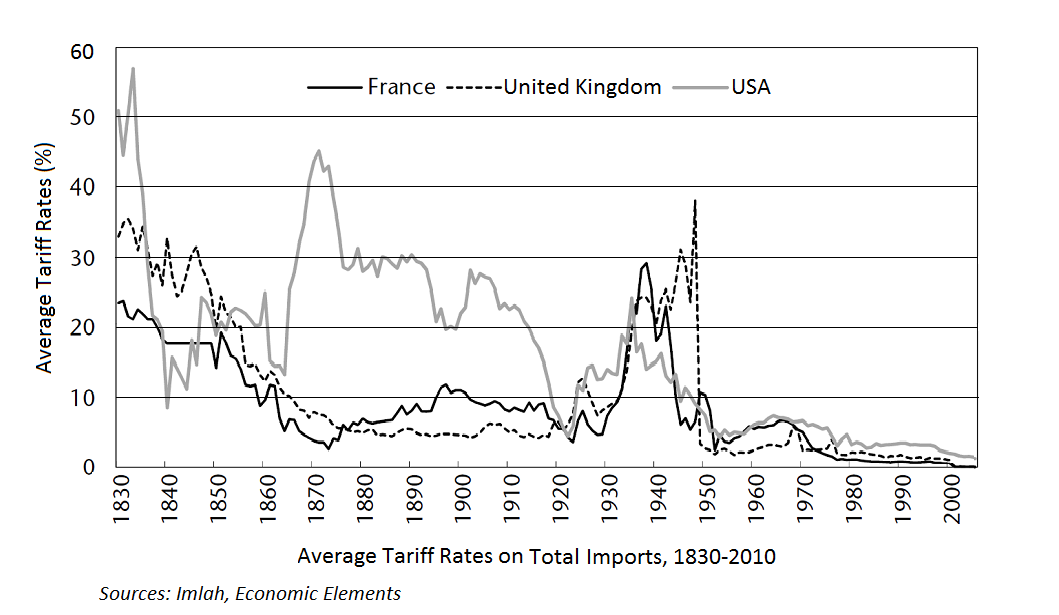
\includegraphics[width=0.7\textwidth]{img/avg_tariff_rates_US_FR_UK.png}
        \caption{Source: Wikipedia based on Albert Imlah's \textquote{Economic Elements}}
        \label{fig:average_tariffs_history}
    \end{figure}
    
    Albeit these tariffs have greatly decreased, many still exist in order to protect some at-risk domestic productions. However, nowadays, countries living in autarky (e.g. self-sufficient) are close to non-existent. Even North-Korea trades goods and services with countries such as Russia or China for instance.
    
    Today, the tariff rates all around the world vary from 0\% to roughly 20\%. A map summarising the average weighted tariff rate applied across all products is presented in Figure~\ref{fig:world_bank_tariffs}. This map is openly available on the World Bank's website\footnote{\url{https://data.worldbank.org/indicator/TM.TAX.MRCH.WM.AR.ZS?end=2018&start=2018&view=map}}.
    
    \begin{figure}[H]
        \centering
        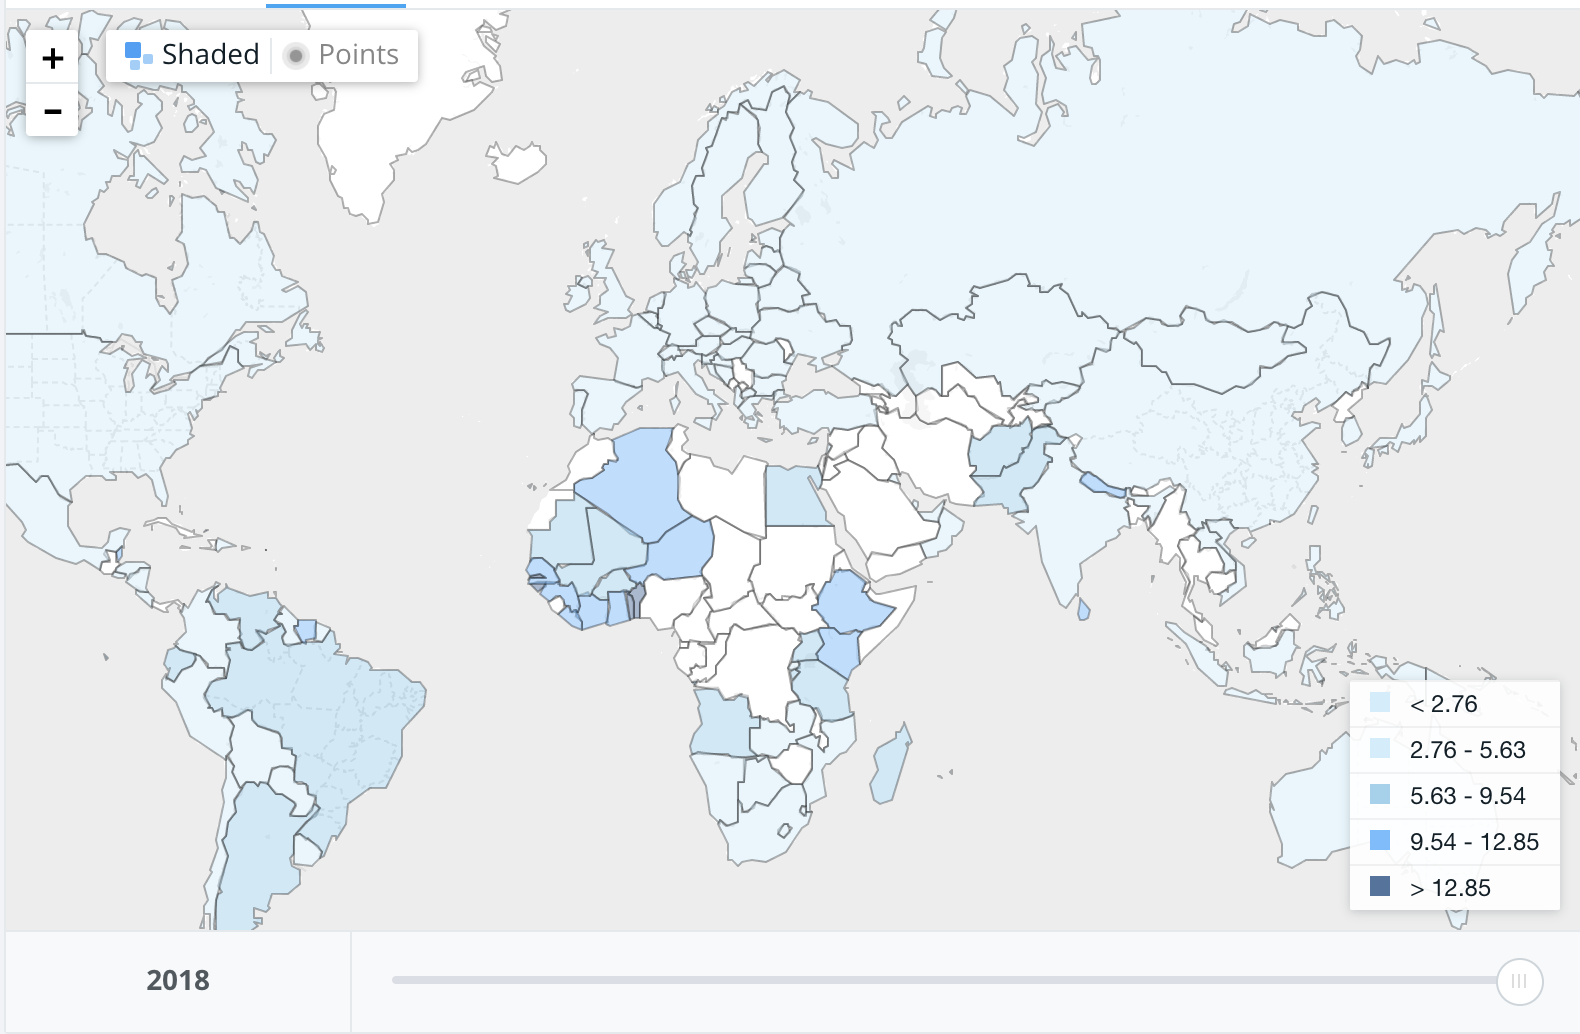
\includegraphics[width=0.7\textwidth]{img/world_bank_tariffs.jpg}
        \caption{Source: World Bank Data}
        \label{fig:world_bank_tariffs}
    \end{figure}
    
    Finally, we will note one very interesting case which is the tariffs rates of small countries, such as remote islands. "The Modern VAT" (\cite{TheModernVAT}) suggests that the advantages of a VAT will be greater than those of a tariff because of the large amount of imports.
    
    
    \subsubsection{Levy (contribution)}
    
    This levy tax can be seen as the income tax in the real world. Nevertheless, the levy tax in our model will be much simpler than the income tax which is a tax based on the income of a year, a time measure which does not exist in our timely discrete World made of ticks.
    
    This tax targets the income and profits earned by an agent, usually during a one-year period. This tax has been around for much longer than the VAT for instance as it appeared in the United Kingdom as early as 1799. In the great majority of the world, this tax is paid by an agent to the State in which it resides. It may be different in some countries (for example in the USA which taxes its citizens, even the non-residents ones), but this particularities go beyond our simulation which only knows the concept of residents.
    
    The income tax can usually be classified in one of the following categories:
    
    \begin{itemize}
        \item Proportional (or flat). In this case, the tax rate is constant across all income levels. The same marginal rate is applied no matter how much income is declared by an agent. Countries applying this kind of taxation include Romania, Russia, or Hungary. Some US states also collect a flat tax (in addition to the federal progressive tax).
        
        \item Progressive. In this case, the tax rate will increase as the income increases (by stages). This is the most used taxation category among the three. As shown by Giacomo Corneo \cite{progressive_taxation}, \textquote{tax progressivity might improve efficiency and the more so in egalitarian  economies}. Indeed, the poorer agents will usually pay a smaller tax rate whereas the richest agents will pay a higher a levy at a higher taxation rate. One should be careful, this is different from a wealth tax which is introduced in the next section~\ref{section:wealth_tax}.
        
        \item Regressive. Contrariwise to the progressive tax, this tax imposes a a greater burden on poorer agents. There are very few examples of such taxation systems.
    \end{itemize}
    
    As usual, the rates will greatly depend from one country to another. Some countries such as the United Arab Emirates do not levy any income tax whereas some countries can collect up to half of the gross income in taxes such Denmark or Belgium.
    
    \subsubsection{Wealth tax}\label{section:wealth_tax}
    
    The wealth tax is a taxation on the assets held by an agent. In our case, we will only take into account the financial assets, and more precisely the money an agent has in its "bank account".
    
    It is, once again, another tool that a State can use to increase its revenues. The idea of a wealth tax is as old as the Ancient Greek civilisation. Indeed, the symmoria \footnote{\url{https://en.wikipedia.org/wiki/Symmoria}} were a group of wealthy citizens that were grouped together with the purpose of collecting a higher tax: a wealth tax to put is simply.
    
    Nowadays, a wealth tax is present in several countries, but it not as generalised at other taxes such as the ones we have previously mentioned. This wealth tax is generally described as a certain percentage of the asset's which has to be paid to the State if the total amount of the assets exceeds a certain threshold. Multiple thresholds can be defined in order to have a progressive wealth tax. For example, taxing 2\% for assets worth more than \$50.000.000 and 6\% for assets worth more than \$1.000.000.000 (1 billion dollars). These are the numbers cited by US senator Elisabeth Warren \footnote{\url{https://www.cbsnews.com/news/elizabeth-warren-wealth-tax-who-would-pay-and-how-much/}}. However, a wealth tax can introduced starting much lower amounts. In Spain for example, the wealth tax starts gradually from 700.000\euro \footnote{\url{https://www.spanishpropertyinsight.com/tax-and-pensions/spanish-wealth-tax-patrimonio/}}.
    
    A huge drawback of the wealth tax is tax evasion and tax havens. Our imperfect simulation will not be able to take these into account unfortunately. According to Åsa Hansson, such a tax could dampen economic growth by reducing the level of investment. However the impact would be very limited.\cite{hansson2010wealth} Again, our imperfect system is not able to model investment and R\&D, therefore, the results in our simulation might be very different.


\subsection{Parameters which the State has direct no leverage on}
    
    As mentioned earlier, there are some key parameters, or rates, which the State cannot influence \emph{directly} contrariwise to the taxes rates. We will dive into two significant rate which have an important role in a economy: the black economy share, and the unemployment rate.

    \subsubsection{Black economy}
    Black economy, also known as shadow economy or non-observed economy \cite{oecdBlack}, is a part of the economy which goes ``unseen'' by the State, usually in order to avoid paying due taxes. One can also note that the formal standardized definition does not include illegal activities (such as drug selling or prostitution) in the black economy share. \cite{pyle1989tax} 
    
    Avoiding paying such taxes allows, on the one hand, the agents to pay less money for their products, therefore being able to buy more products. However, on the other hand, the State will see its taxes revenue decrease. 
    If black economy is limited, then its impacts may be negligible. However, if the black economy takes a large part of the total economy, the State will not be able to play its redistribution role resulting eventually in more inequalities among the agents. As noted by Anna Krajewska, one big disadvantage of this underground economy is the ``deepening [of] income differentiation''. Contrariwise ``high  taxes  and  transfers  lead  to  more  equal  distribution  of incomes.'' \cite{blackEcoImpact} We will see in our experiments what role this rate plays regarding different metrics including the income difference between agents (Gini coefficient).

    Unfortunately, the black economy is hard to measure precisely. Economists have come up with different kind of methods to evaluate this share such as sampling a portion of the population tax returns and analyze them thoroughly. From this, one can extrapolate the results to a larger scale. \cite{pyle1989tax}. This non-observed economy share has been estimated for several countries, among which some countries of the OECD (Organization for Economic Co-operation and Development) as presented in the figure~\ref{fig:black_economy_oecd} below. It is computed as a share of the total GDP of the country. For instance, Belgium sits at around 22\%. This is a rather significant estimate.
    
    \begin{figure}[H]
        \centering
        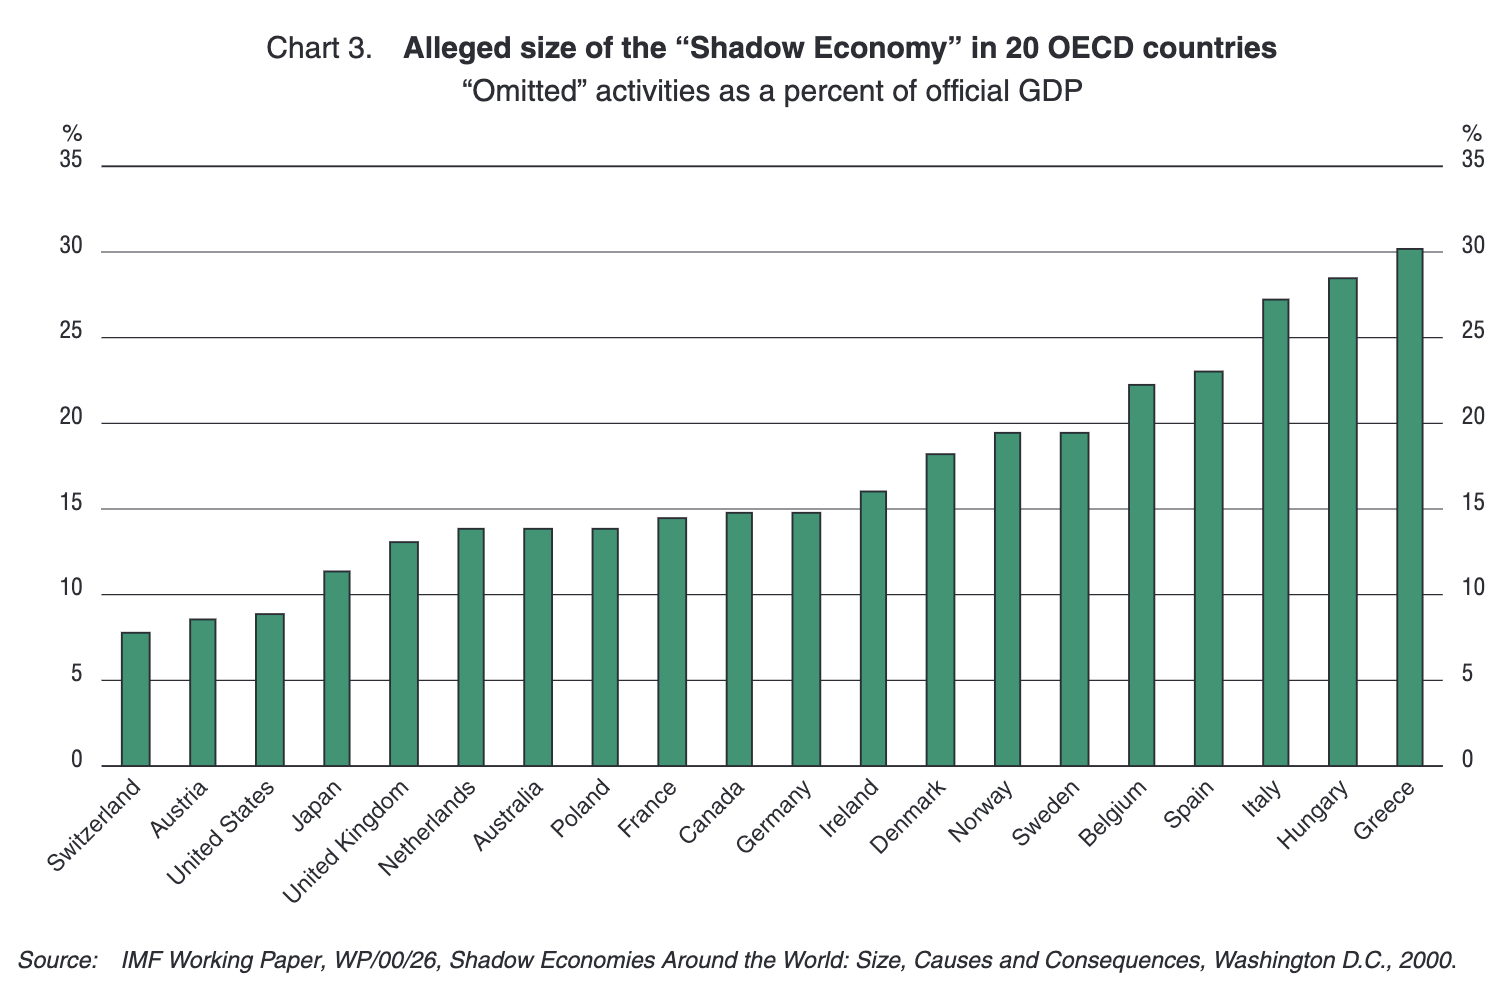
\includegraphics[width=0.8\textwidth]{img/black economy OECD.png}
        \caption{Source: \cite{oecdBlack}}
        \label{fig:black_economy_oecd}
    \end{figure}

    \subsubsection{Unemployment}
    The second rate which the State cannot \emph{directly} control is the unemployment rate. This rate is defined as the share of active people (usually adults in age of working) who have no money-making activity and therefore no direct revenue. 

    Naturally, the higher the unemployment rate is, the less money the State will collect from taxes. In such a case, the State will have less money to redistribute through allowances hence inequalities will more prevalent among agents. This has been studied by H. Naci Mocan where he draws the conclusion that ``decomposition  of  unemployment  into  cyclical  and  structural  components  reveals  that  an  increase  in  structural unemployment  increases  the  income  share  of  the  highest quintile, and decreases the shares of the bottom sixty percent of the population.'' \cite{Unemployment1}, in other words the inequalities are much more prominent and the Gini coefficient is therefore higher. These results have been confirmed by another researcher Rubens Penha Cysne who analyzed, empirically, standard job-search models, and found a ``positive correlation between inequality and unemployment'' \cite{Unemployment2}. Therefore, these two will be important parameter and metric to analyze later on in our experiments.

    In June 2021, in the OECD, the average unemployment rate was around 6.6\%, which is a bit (1.3\%) higher than before the COVID-19 pandemic. In Belgium, the rate is around 5.3\% (and 5.0\% in February 2020 before the pandemic).
    \footnote{\url{https://www.oecd.org/newsroom/unemployment-rates-oecd-update-june-2021.htm}} We can see the evolution of this metric on the following figure~\ref{fig:unemployment_oecd}.
    
    \begin{figure}[H]
        \centering
        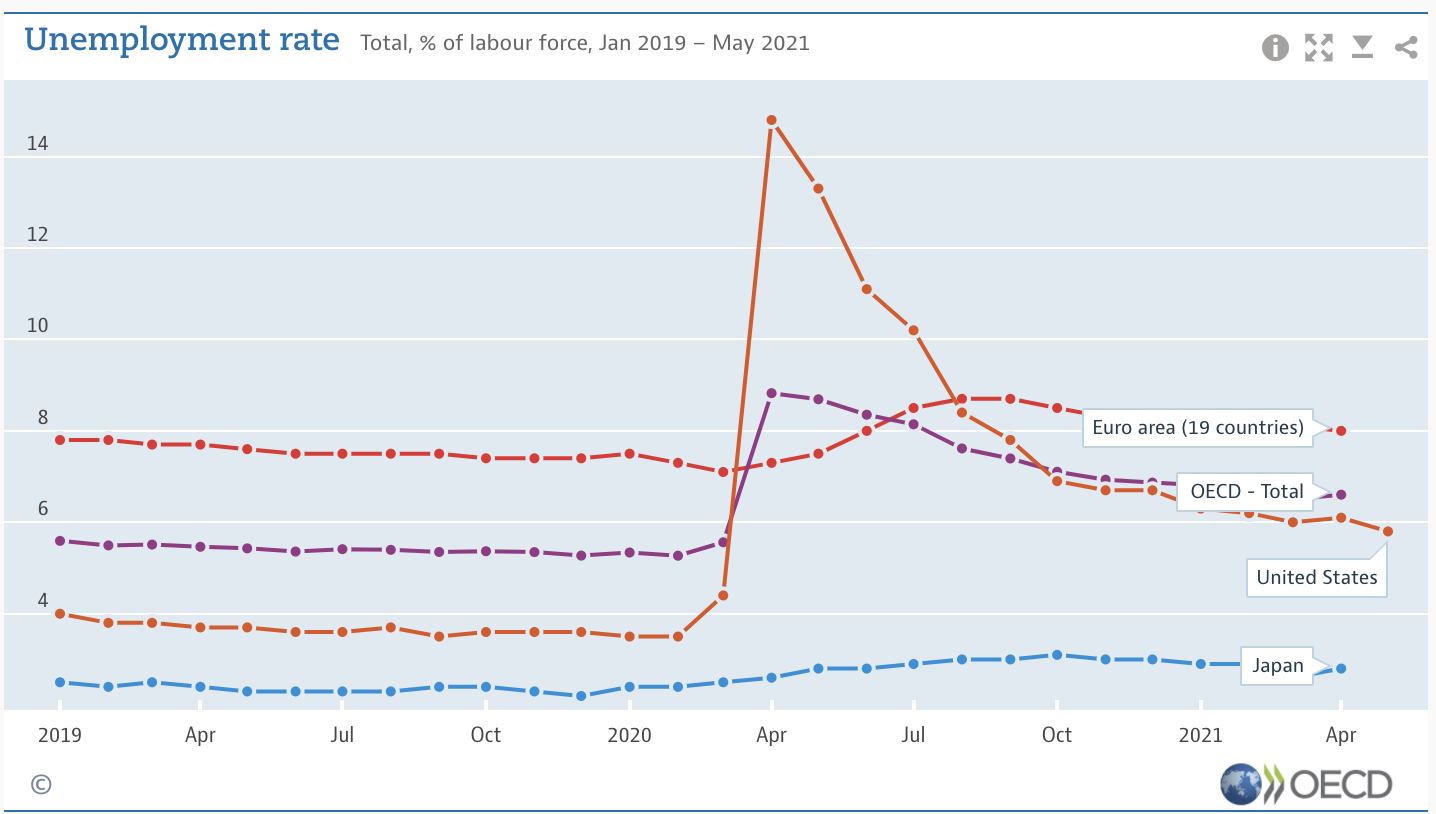
\includegraphics[width=0.8\textwidth]{img/unemployment_OECD.png}
        \caption{Source: OECD website}
        \label{fig:unemployment_oecd}
    \end{figure}



\subsection{Allowance and Universal Basic Income}

Because the State has collected money from different taxes, it will now have to redistribute it. In our simulation, there will not be any infrastructure or services that the agents can take advantage of such as public roads or free education. Therefore, all the money levied through taxes will go fully to the wealth distribution system which can be of two types in our system: either through allowances, or through the universal basic income (UBI). It is a exclusive choice, it is either one or the other, not both. So each fictional State will have to make a choice.

    \subsubsection{Allowance}
    
    An allowance is an amount of money given by a State to some of its citizens under certain conditions. The system handling this is called the social security whose role is to provide money to the less fortunate citizens. It insures that every citizen can afford, at least, the most basic needs such as food or shelter. Poorer people will usually receive more money than the wealthier who can already afford a better lifestyle.
    
    However, social security is not always a right in every country. Not all countries have implemented this safety net. According to the United Nations, the majority of the people across the world are not protected by a social security \footnote{\url{https://news.un.org/en/story/2010/11/359142-un-study-finds-most-people-worldwide-have-no-social-security}}. This social security is mostly available in developed countries whereas the percentage of people covered by such a system falls to around 5\% in sub-Saharan Africa.
    
    In our simulation, the social security will be a way of redistributing wealth in order to allow every agent to produce and consume products.
    
    \subsubsection{Universal Basic Income}
    
    Contrariwise to the allowances, in the universal basic income, we give the same amount of money regardless of the situation of each citizen. Therefore, UBI is actually a particular case of the general allowance. Everybody receives this amount of money periodically, no strings attached. The idea of a guaranteed income has been proposed throughout history (as early as the 16th century) and some countries have tried it but only for a limited period of time and only for a small sample of the population. Examples of countries that have tried UBI include Kenya, Finland and Macao but at a relatively limited scale. 
    
    According to its advocates, the main reason why UBI will be necessary sooner or later is because of the rise of technologies which will replace humans and therefore making them jobless. Its ultimate goal would be to eradicate poverty by assuring everyone a decent amount of money for the most basic needs. And although it might seem Utopian and perhaps not perfect, Thomas Straubhaar, argues that it is worthwhile.\cite{straubhaar2017economics}
    
    However, its detractors critic the cost of such a system and its viability. Another argument is that, although some jobs will be lost, new ones will probably be created; the same way it was done during the industrial revolution. Finally, according to the critics, it is unfair because even the richest people would get this income. Robert Stephens rather suggests \textquote{to simplify and amend the current system, to make it fit  better  with the realities of the 21st century} \cite{stephens2019universal}. One might also critic its purpose since the goal of the redistribution is to diminish inequalities, which will hardly be the case if every agent receives the same amount of money. We will analyze and compare these two ways of distributing wealth and see which one performs better on which metrics.

    
\subsection{Economic clusters}
    As we have seen before, countries can impose tariffs on customs in order to discourage imports and encourage local consumption. However, what if countries had agreements between them in order to allow free trade (thus a null customs tariff) in-between a cluster? The most simple cluster would be made of two States freely importing and exporting from and to one another. This is known as a bilateral agreement. However, we can extrapolate this idea to more countries: a cluster made of a single market where no import tariffs would be levied by its member states.
    
    A very famous real-world example is the European Union (EU). The EU currently counts 27 member states exchanging in one single market with no tariffs on customs. The EU holds lots of advantages among these we can cite a few such as the freedom of movement or worker's protection across all member states, and the most important one being the large common market where goods and services can be exchanged at a cheaper price because of the lack of tariffs which also encourages investment.
    
    It also has some drawbacks such as the membership cost, the non-unique currency, and more bureaucracy. However, these will not be present in our simulation which does not model these aspects.
    
    We should also note that being in a cluster does not exclude a member state from having other bilateral agreements with other states. Indeed, the difference between the two is that a bilateral agreement is only between two countries, whereas in a cluster, all States are connected to one another. We will see how these two will influence important metrics such as the number of transactions or the Gini coefficient.

\subsection{Efficiency/Equality trade-off}
    Finally, we will briefly discuss the broad question of the efficiency/equality trade-off and why it is a trade-off. Indeed, a trade-off means that improving one side will, generally, deteriorate the other side.
    
    This trade-off has actually been studied in previous works related to this one with the original work being the one of Bersini and van Zeebroeck: \textquote{Why should an economy be competitive ?}. This publication concludes that \textquote{a competitive market distributes welfare much less equally and is responsible for inequality amplifying effect} \cite{bersini}. We will also do an empirical analysis of this trade-off and analyze the results computed by our simulation.
    

\section{In computer science}

    \subsection{Computer simulation}

    Computer simulations have been around for almost as long as computers themselves. They are a tool with a great interest in Science as they have been used in all possible scientific domains. They allow to validate or reject an hypothesis of a research question if they are precise enough. Indeed, whenever an analytical method is not imaginable because of its complexity, we can use a computer simulation to perform the computations at the cost of the precision of the results. However, with models accurate enough, important amount of data, sufficient computational power and run time, one can get very close to the exact results. \cite{exprimentationNumeriqueParOrdinateur}

    Nowadays, they are used in almost all domains: biology, physics, climatology, economics, ... They can be used to validate results of an experiment, simulate a real phenomenon and understand its models and parameters (which we are going to do in this thesis), make predictions for future events, try a potential model on a computer before putting it in the real life... The use cases are endless. They are a quite cheap way (compared to other methods) to do all these things and allow us to test some models before doing important investments.

    There are lots of examples in our society where computer simulation are used daily. For instance in weather forecasting, power distribution and needs, traffic engineering, aerodynamics of car models, fluids, etc. These state-of-the-art examples (which actually get better and more precise everyday) come from different fields of science and engineering. \cite{weatherForecasting} Some people even argue \emph{we} actually live in a simulation...

    \subsection{Agent-based modelling}
    Agent-based modelling (ABM) relies on computer simulation as we simulate lots of independent and heterogeneous agents (commonly, an agent represents a person, however it can also represent an entity such as a State) that interact with one another. As the simulation goes on and entities interact, we will be to see some patterns emerge and therefore study the parameters that have led to such patterns. Usually, lots of simple entities will lead to interesting phenomena on a large scale and, naturally, the more entities/agents we have in our simulation, the more accurate our results will be (at the disadvantage of having a longer run-time). Thus, the interactions happening between micro-structures (our agents/entities) allow us to see patterns at the macro level (an economic system for instance).
    
    This is presented by Prof. Bersini as ``Weak emergence''.\cite{ctaiABMBersini} A simple example of this is life. ``Living cells are made of mineral particle, yet, it impossible to find characteristics of life in the simple components of these particles such as atoms of hydrogen, oxygen, carbon, and nitrogen''. Therefore, ``life is in the whole, not the parts'' as Durkheim concludes. \cite{ctaiABMBersini}.

    There are three main types of ABM \cite{ctaiABMBersini} :

    \begin{itemize}
        \item Automata: they are the simplest kind as they only repeat a set of (simple actions without any kind of knowledge. 
        \item Interested: they are a bit more advanced as they make biased choices. For instance in game theory, we might prefer one action over another depending on a payoff matrix.
        \item Adaptive: they try to learn as the simulation runs in order to adapt and maximize some kind fitness.
    \end{itemize}

    Furthermore, as shown by Prof. Gallegati, ``aggregation generates regularities''. This means that every single agent does not to be stable, because when we aggregate all of them through the simulation, stable ``statistical regularities [will] emerge from individual disorder''. \cite{MauroGallegati}

    As for computer simulations, ABM is a very interesting tool to detect weak emergence and understand how it emerges. By understanding how it emerges, we are also able to make better predictions by changing some components and see the output. Finally, according to these predictions, one can make decisions and regulate the key parameters when transposing the computer simulation into real life. \cite{ctaiABMBersini}

    %\subsection{Optimization}
        %TODO

\chapter{Simulation}

\section{Parameters}

All parameters of the simulation have been regrouped into a single configuration \texttt{JSON} file with a hierarchy based on the models (each one will read the values it needs). Whenever we are testing one configuration of the simulation, we can simply modify the values of this file to see the consequences of such modifications compared to the template version (\texttt{params/templateExperiments.json}). The default file looks like as shown in the following figure and all parameters will be explained in the following sections.

\begin{lstlisting}[language=json,firstnumber=1]
{
    "World": {
        "PRODUCT_CHOICE": "CHEAPEST",
        "NB_STATES": 200,
        "NB_AGENTS": 30000,
        "NB_TICKS": 4000,
        "NB_TICKS_SAVE_CSV": 100
    },
    "Connections": {
        "CLUSTER_SIZE": 0,
        "PROB_CONNECTION": 0.0
    },
    "State": {
        "Tax": {
            "MIN_VAT": 0.2,
            "MAX_VAT": 0.2,
            "MIN_LEVY": 0.1,
            "MAX_LEVY": 0.1,
            "MIN_TARIFF": 0.3,
            "MAX_TARIFF": 0.3,
            "VAL_WEALTH_TAX_TOP": 0.1,
            "MIN_WEALTH_TAX_VALUE": 0.2,
            "MAX_WEALTH_TAX_VALUE": 0.2,
            "NB_TICKS_COLLECT_TAXES": 100
        },
        "Allowance": {
            "NB_TICKS_DISTRIBUTE_ALLOWANCES": 100
        },
        "Others": {
            "MIN_UNEMPLOYMENT": 0.05,
            "MAX_UNEMPLOYMENT": 0.05,
            "MIN_BLACK": 0.15,
            "MAX_BLACK": 0.15
        }
    },
    "Agent": {
        "MIN_INIT_MONEY": 1000.0,
        "MAX_INIT_MONEY": 1000.0,
        "RATIO_BUY": 0.5,
        "RATIO_PRODUCE": 0.5
    },
    "Product": {
        "NB_DIFF_PRODUCTS": 50,
        "MIN_PRICE": 0.0,
        "MAX_PRICE": 300.0,
        "MAX_STOCK": 2000
    }
}
\end{lstlisting}

\section{Main}

    The simulation has been coded using Java 16 for its large range of libraries, robustness, rapidness (compared to Python for instance), its strongly typed paradigm and, of course, because of its Object Oriented Programming paradigm (OOP) which fits how we will code our models (see next section). 

    Everything starts with the \texttt{Main.java} file. Multiple simulations can be ran in parallel thanks to the use of threads (one simulation = one World = one thread). Each line in the \texttt{params/configs.txt} file corresponds to one configuration (thus one \texttt{.json} file containing all the parameters located in the \texttt{params} directory) that will be launch. For instance:

    \begin{lstlisting}[language=json,firstnumber=1]
experiment1.json
experiment2.json
experiment3.json
    \end{lstlisting}



\section{Models}\label{section:models}

ABM provides numerous benefits, as stated before. Amongst these, we can cite two key points that motivate this thesis: \textquote{ABM captures emergent phenomena and it provides a natural description of a system}. This is important because our goal is to have an empirical understanding of our system \cite{tesfatsion_handbook}, i.e., we want to understand why some systems work while others do not. And this will be done with in very intuitive way based on a natural description of ours models which will interact.

Nonetheless, we should also note some drawbacks of this approach; especially the issues revolving around social sciences such as irrational behavior or subjective choices which are difficult to quantify and pin down mathematically \cite{ABM}. In order to simulate some irrational behavior, we could introduce some non-deterministic behavior where the agents would make a random choice from time to time. However, such a stochastic behavior will be hard to calibrate. 
Another problem that may rise is the required computational power. Simulating such a complex system made of different models with many thousands agents is expensive. Therefore, we shall use tools that allow us to perform heavy computations as described in the implementation section~\ref{section:implementation}. 

We will now focus on the different models that make up our economical system: the World, the WorldMarket, the States, the Market, the Agents and the Products. We will start by the smallest entity until the biggest: from Products to the World.


\subsection{Product}\label{section:product}
In the real world, we have two different types of products: the goods and the services. However, in this paper, we will not distinguish these two terms because the only thing that matters is that one producer and one consumer perform an exchange of a product in return of a certain amount of money. From now on, we will use the word \emph{product} to encompass these two words.

Each Product belongs to one Agent has a type (which is a simple number) to represent different kinds of products (apples, clothes, cars, ...), a default selling price (which will be updated by the Agent according to its skills) and the stock units.

We should also note that by "exchange of product", we mean a sale-purchase relationship: after receiving the money, the producer does not have any right on the sold product anymore as opposed to a location or a license. We also assume that any product sold is directly consumed by the buyer.

\subsection{Agent}\label{section:agent}
We will focus on four key aspects of an agent: its assets, its actions and its skills. Each agent is unique. This will allow us to have an heterogeneous 'society' similarly to the one in which we live where each and every one of us has some assets and different skills.

    \subsubsection{Assets}\label{section:assets}
    Usually an agent owns multiple and different types of assets. In our case, we will focus on the financial and material ones. Indeed, an agent has a certain amount of money on its bank account. This amount is, needless to say, variable. 
    However, each agent will start the simulation with a certain amount of money and afterwards, it will be up to it to spend it as it wishes and also increase it by selling the products it produces (see section about skills~\ref{section:skills}). 
    The amount of money an agent has will play a key part in the statistics that we will compute in order to study our study (for example to study the wealth distribution amongst agents). 

    Our agent will also have material assets, namely the products it produces. It can only produce one type of products as described in section about skills~\ref{section:skills}. By producing a unit of a certain type of product, we increase the stock the agent has of that product. And, similarly, by selling a unit of a product, we decrease the stock if it was not empty. We can note that there is a lower bound (0 unit), and an upper bound depending on the parameter \texttt{Product.MAX\_STOCK}.


    \subsubsection{Actions}\label{section:actions}
    An agent can be seen as a person who has both duties and rights. The agent \emph{can} produce, make a transaction (which encompasses the selling and buying actions) and consume products. These actions belong to the rights of the agent. Performing any of those actions will involve different components: a product, some money, a buyer (or consumer) and a seller (or producer) and the States to which our agents belong. 

    However, we should also note that an agent has duties. Indeed, in our system we will introduce the concept of State (in the section~\ref{section:state}). Because an agent belongs to a State, it \emph{has} to pay certain taxes. 
    For instance, the well-known VAT (Value Added Tax) which has to be payed to the State each time an agent \emph{sells} a product. The rate the VAT will be State-dependent. Depending on the State, we may have different taxes that we will study to see how they influence our system. All these taxes are examples of duties an agent has. 

    The actions involving a product are described as followed:

    \paragraph{Produce}
    Producing is the primary goal of an agent. At first, the Agent chooses one Product type to produce. Depending on its \emph{talent} (a random value between 0 and 1), the Agent will be able to reduce the default selling price of that product as: 

    $$Product.sellingPrice = (1-talent) \cdot Product.defaultSellingPrice$$

    So the more talent an agent has, the smaller the price of the product will be and therefore the more chances this product will be bought by other agents. On the other side, it has decided that there are no production price because otherwise, tick after tick, money would 'leak' out of the System until no agent is able to buy or produce which would be counterproductive for the experiments.

    However, an agent will not be able to produce at each time step (a tick as described in section~\ref{section:world}). This will allow other agents (buyers, i.e., consumers) to have some time to buy our agent's products. Indeed, our agent should not produce all the time in order to avoid having too many stocks of unsold products. An agent will not be able to produce indefinitely, we have an upper bound: the max stock allowed by the parameters (\texttt{Product.MAX\_STOCK}).

    \paragraph{Buy} 
    An agent does not buy at every time step (tick), but when it does, it will analyse all its possibilities. It will choose one product it needs and try to find a seller. For this, we will analyze all the sellers and rank their products by price. This will be detailed in the Market section.


\subsection{State}\label{section:state}
In this work, we introduce a new concept of 'State' which we will define as an entity containing multiple agents constituting a community operating on the same sets of rules.

    \subsubsection{Rights and duties}
    All of the agents in our simulation will be assigned to only one State: an many-to-one kind of relationship (multiple agents belong to one State). As stated previously, agents have some duties towards the State they belong to: taxes.

        \paragraph{Duties}
            Whenever an agent sells a product to another agent, it has to pay a certain amount to the State to which it belongs. This is an already existing concept: the Value Added Tax (VAT). This amount is computed as a percentage of the product's price. The VAT's value will be decided by the State. Other taxes have been introduced too:

            \begin{itemize}
                \item the levy which is a contribution to the State. This levy will happen every time a certain number of ticks have been performed. The amount of this levy is fixed according to a certain percentage of the financial assets of an agent.
                \item custom tariffs which will discourage buying from non-connected States as they penalize the price of a Product sold by another State with which there is no connection.
                \item a wealth tax which will not be payed by all agents, only the wealthiest. This tax is optional and not all States will impose it. It will be obligatory for the top 10\% richest agents.
            \end{itemize}

            The default values of these taxes were chosen to be close to the averages of the OECD's.

        \paragraph{Rights}
            However, they also have some rights in regards to the State that are split in two categories: allowances and a universal basic income (which is in fact a particular case of allowances). Each State may choose to use exclusively one of them.

            \subparagraph{Universal Basic Income}
                The simplest case is the universal basic income which does not make any distinction between the agents. Every agent belonging to the same State will receive the same amount of fictional money (what is called the \texttt{Flat} allowance in the code). Therefore we simply divide the money of the State by the number of agents it has and every agent receives the same share of money.
            

            \subparagraph{Allowance}
                The amount of an allowance will depend greatly on the wealthiness of its receiver because its goals is to distribute wealth (what is called the \texttt{Fair} allowance in the code). To compute the amount that each Agent receives, we have to take into account the following three conditions:
                
                \begin{itemize}
                    \item The State cannot distribute more money than it has
                    \item The wealthiest agents should still be wealthier (thus, the order of agent's wealth should stay the same, i.e. the poorest agent cannot suddenly become the richest after allowances have been distributed). 
                    \item Wealth is distributed more evenly among agents.
                \end{itemize}

                For this, I have decided to use the following methodology:

                \begin{enumerate}
                    \item Compute the average money of an agent
                    \item Compute, for each agent, the difference between its money and the average. If the Agent has more money than the average, the difference will be set to zero.
                    \item Now we know how much money the State has to distribute. However we have two cases that might happen: either the State has enough money, or not.
                    \item If the State has enough money, we simply give each Agent its computed difference with the average, and divide the rest of the money the State has equally between all agents.
                    \item If the State has not enough money, we compute the share of an agent based on a simple computation: $\frac{\text{stateMoneyToDistribute} \cdot \text{difference}}{\text{totalToDistribute}}$. This guarantees the State does not spend more money than it has, while reducing inequalities.
                \end{enumerate}

                \subparagraph{Example}
                The State has 100 units of money to distribute among 4 agents. Currently, A is the poorest and has 10 units of money, B 20, C 100 and D 170. The Gini coefficient is equal to 0.467 and the average money of an agent is therefore $\frac{10 + 20 + 100 + 170}{4} = 75$. Hence A's difference is thus $75-10=65$, B's 55, C's 0 and D's 0. However, the State does not have sufficient money to pay both A and B (total of 120, yet the State has only 100). Thus, A will receive $\frac{100 \cdot 65}{120} \approx 54.1$, and B $\frac{100 \cdot 55}{120} \approx 45.8$. The total distributed money is therefore 100, and the inequalities between agents has been reduced: A, B, C have 100, D has 170. This respects our three conditions from earlier and the Gini coefficient is equal to 0.112 (closer to 0 means more equality)


        \paragraph{Wealth distribution}
        The taxes and allowances are introduced in order to limit the money difference between the richest and poorest agents and allow a better distribution of the wealth in the system. Because all these parameters are adjustable, different type of States will emerge.

        Traditionally, States can, very roughly, be divided in three categories: pure socialism, pure capitalism or mixed. If a State decides to collect no taxes and offer absolutely no wealth distribution, we would label it as a pure capitalist economy. Conversely, if a State decides to opt for a planned economy (or pure socialism), every agent would work for the State it belongs to, and would not be able to increase its own financial assets because the taxes are too high for instance in our simulation.
        However, most real markets today are not that extreme and fall into the mixed market category where some wealth distribution is present. This is a very simplified classification but it will suffice in our case to study and understand our simulation.

        Wealth distribution will be one of the key factors when we will analyse the simulation.


    \subsubsection{Black economy}
    The black economy is a share of the economy from which the State gets no tax. This is a parameter of the System and each State has one value in between 0 and 1 (e.g. 0.2). Thus, whenever one of its agents makes a purchase, it will not, according to a certain probability defined by the State, pay VAT, nor augment the GDP of the State. However, agents will still pay the levy and the wealth tax (for those concerned about it).

    \subsubsection{Unemployment}
    Another interesting parameter is the unemployment rate. It is also a parameter of the System and each State has one value in between 0 and 1 (e.g. 0.2). According to this probability, some agents of the State will simply never produce during the course of the simulation. This is a probability, therefore, if the State has 100 agents and an unemployment rate of 0.2, \emph{around} 20 agents will not produce.



\subsection{Connections}\label{section:connections}
    The World we live in is very connected: States are very connected to one another and lots of exchanges take place across two different States. However, in our simulation, we will not connect them all in order to study the globalization phenomenon and the importance of custom tariffs. 

    In our simulation, when two States are connected, we mean that a transaction may happen between a seller of one State A and a buyer from a State B without any custom tariff. However, if they are not connected, there will be a custom tariff on the sale which varies from State (\texttt{parameter State.Tax.TARIFF}). 

    An interesting form of connection that might happen will be clusters: groups of inter-connected States. Such clusters happen in real life such as the European Union where no custom taxes are collected when a transaction happens between a seller and a buyer from two different States. The same will apply in our simulation. 

    The difference between connections and clusters is that in a Cluster, all member States are connected to each other. Whereas in the case of a simple connection, it is a simple bilateral connection between those two. For instance, if A is connected to B, and B is connected to C, then we cannot infer that A and C are connected in the case of simple connections. However, in the case of a Cluster, they will.

    Figure~\ref{fig:connected_states} is an example of a graph of States where each vertex represents one State, green edges represent a connection of two States belonging to a cluster and grey edges represent a connection between two States. In this example, we can see that State can have no connection (vertex 0), or that a State belonging to a cluster can still have some external connections to other States which do not belong to the cluster (for example vertex 4 connected to vertices 8 and 12 with a grey edge instead of a green one).

    \begin{figure}[H]
    \centering
    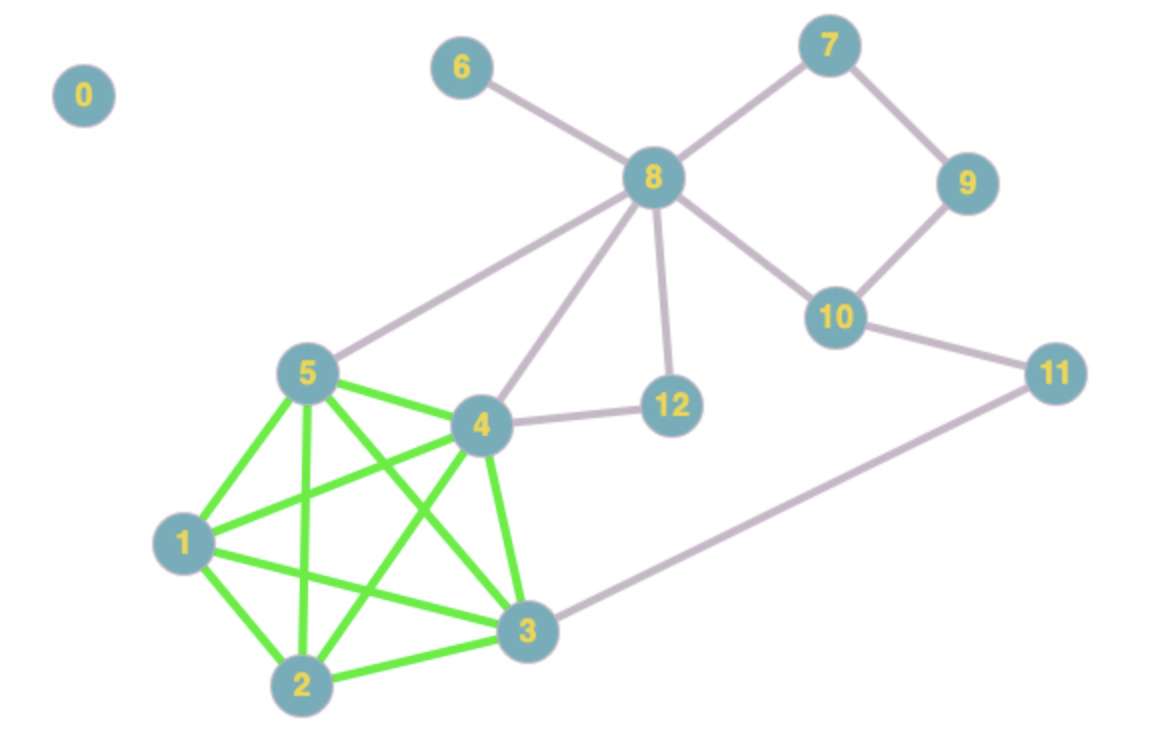
\includegraphics[width=0.7\textwidth]{img/connected_states.jpg}
    \caption{Example of a graph of States}
    \label{fig:connected_states}
    \end{figure}

    In the code, we have two parameters: first we have \texttt{Connections.CLUSTER\_SIZE} and then we have \texttt{Connections.PROB\_CONNECTION}. The former simply States how many States are present in the Cluster (for simpler analyzes later on, we have maximum one Cluster). We will make sure that all those States are correctly connected to one another. The second parameter simply State what is the probability of a State being connected to another when going through all States present in the World (\ref{section:world}). So, for instance, if we have a probability of 0.3, we will go through all the States of the World, and for each State, it has a probability of 0.3 to create a link with another State chosen at random. By doing this, some State will, possibly, be connected multiple times (i.e. two or more connections without being in a Cluster). This is a good thing as it will allow us to see the importance of the number of connections a State has (or whether it is in a Cluster).


\subsection{Market}\label{section:market}
The Market regroups all the products sold by the agents of one State, thus we have one Market for each State. Whenever a transaction takes place, the Market will compute the price of the exchange by including all the taxes (VAT, Tariff if the agents come from two different States which might not be connected). Whenever an agent wants to buy a Product, we will simply scan all the products available in the market and see which ones fit the demand by filtering on the price (buyer must have enough money) and the stocks of the product. To optimize this search, a HashMap has been created such that products are already sorted by their type and the search is, when profiled, \emph{much} faster, especially when we have tens of thousands of agents.

Whenever an agent wants to buy a product, we get a filtered list of all products the agent \emph{can} buy. There are multiple way of choosing a product from this list. Naturally, we could simply choose the cheapest one among those. However, other choosing methods have been developed to compare them. The other two methods are called \texttt{random} and \texttt{weightedRandom}. The former is rather obvious as we simply choose at random. This means that it is possible that the agent chooses the most expensive product (which is still affordable for the agent since the list has been previously filtered). The $3^{rd}$ method is a mix of the other two as we introduce some random but cheaper products have better chances at getting picked. The higher the price of the product, the less chances it will have at getting picked thanks because each product is associated with a probability which is inverse of its price.

\subsection{World Market}\label{section:WorldMarket}
The role of the World Market is simply to connected all the markets of all States because each Market only contains the products of the agents in that State, yet, agents can buy products from other States, which is why we need this link. Thus whenever an agent wants to make a purchase, we scan the markets of all States of the world and get a filtered list of products for each of them and simply combine them all into a single list of products to choose from. The World Market takes care of the transaction, the Gdp, the payments and other variables such as the black economy share depending which States the buyer and the seller belong to. It also allows us to get some interesting statistics such as the total number of purchases/transactions happening in the World.


\subsection{World}\label{section:world}
After describing all our models, we eventually finish with the one that will encompass them all: the World. The purpose of this model will be to initialize all products, agents and States as well as let them be inter-connected through the World Market.

The World will also handle the time step: a tick. Indeed, because computers are discrete machines, we have divide time into time steps (ticks). At each time step, our World will allow agents and States to perform actions such as producing, buying a product, collecting a tax or distributing allowances.

However, as previously expressed, not all agents will perform an action at every tick. Only a certain percentage of the agents will do something: either produce, or buy, or do nothing (in case it has no money to either produce or buy, therefore it waits for someone to buy one of its products or for the State to give him an allowance). However, the action of selling may happen at anytime. This means that an consumer will be able to buy a product from a seller without waiting for him to also perform an action (otherwise, the system would be blocked very often).
This percentage value will be rather small due to the fact that a tick is something that will happen very often.

Finally, because our World contains all of the models we have defined (i.e. the products, the agents, the States and the World Market), it will allow us to have an overview of all that is going on in our simulation. It will also be very useful in order to study the system and make some statistics. To compute these statistics, we will save all the key metrics of the World (e.g. number of transactions at a certain time/tick), the States (e.g. current Gini coefficient of all States), the Agents (e.g. initial and current money) and the Products (e.g. number of purchases and sales). 

These statistics are saved periodically after 100 ticks in case some error appears in the middle of the simulation. They are saved into \texttt{.csv} files which will then be analyzed later on so that we do not have to run the same simulation multiple times. 


\section{Running}
The project is freely available on Github at the following link: \url{https://github.com/RicGR98/MasterThesis}. All information to run the project are available in the \texttt{README.md} file in the root directory. A \texttt{run.sh} bash file has been created to run everything with a single simple command. This file works for local runs and also on the CECI cluster. Indeed, because these simulations are very computationally demanding, we have used the CECI (Consortium des Équipements de Calcul Intensif) cluster, ``funded by the Fonds de la Recherche Scientifique de Belgique (F.R.S.-FNRS) under Grant No. 2.5020.11 and by the Walloon Region''\footnote{\url{http://www.ceci-hpc.be/}}. For this, one has to copy the project files onto the cluster, then run \texttt{sbatch run.sh} and wait for the job to be launched by the cluster and let the simulation run for minutes, hours, or days (maximum 2) depending on the number of agents, states and ticks parameters. All commands to copy the files are available, as comments, at the end of the \texttt{run.sh} file.


\section{Class diagrams}

    To better understand how everything is linked and structured, we present now some class diagrams (from a large overview to a more detailed view). The class diagrams presented here are only for the Java code (thus for the simulation, not the experiments for instance)


    \begin{figure}[H]
        \centering
        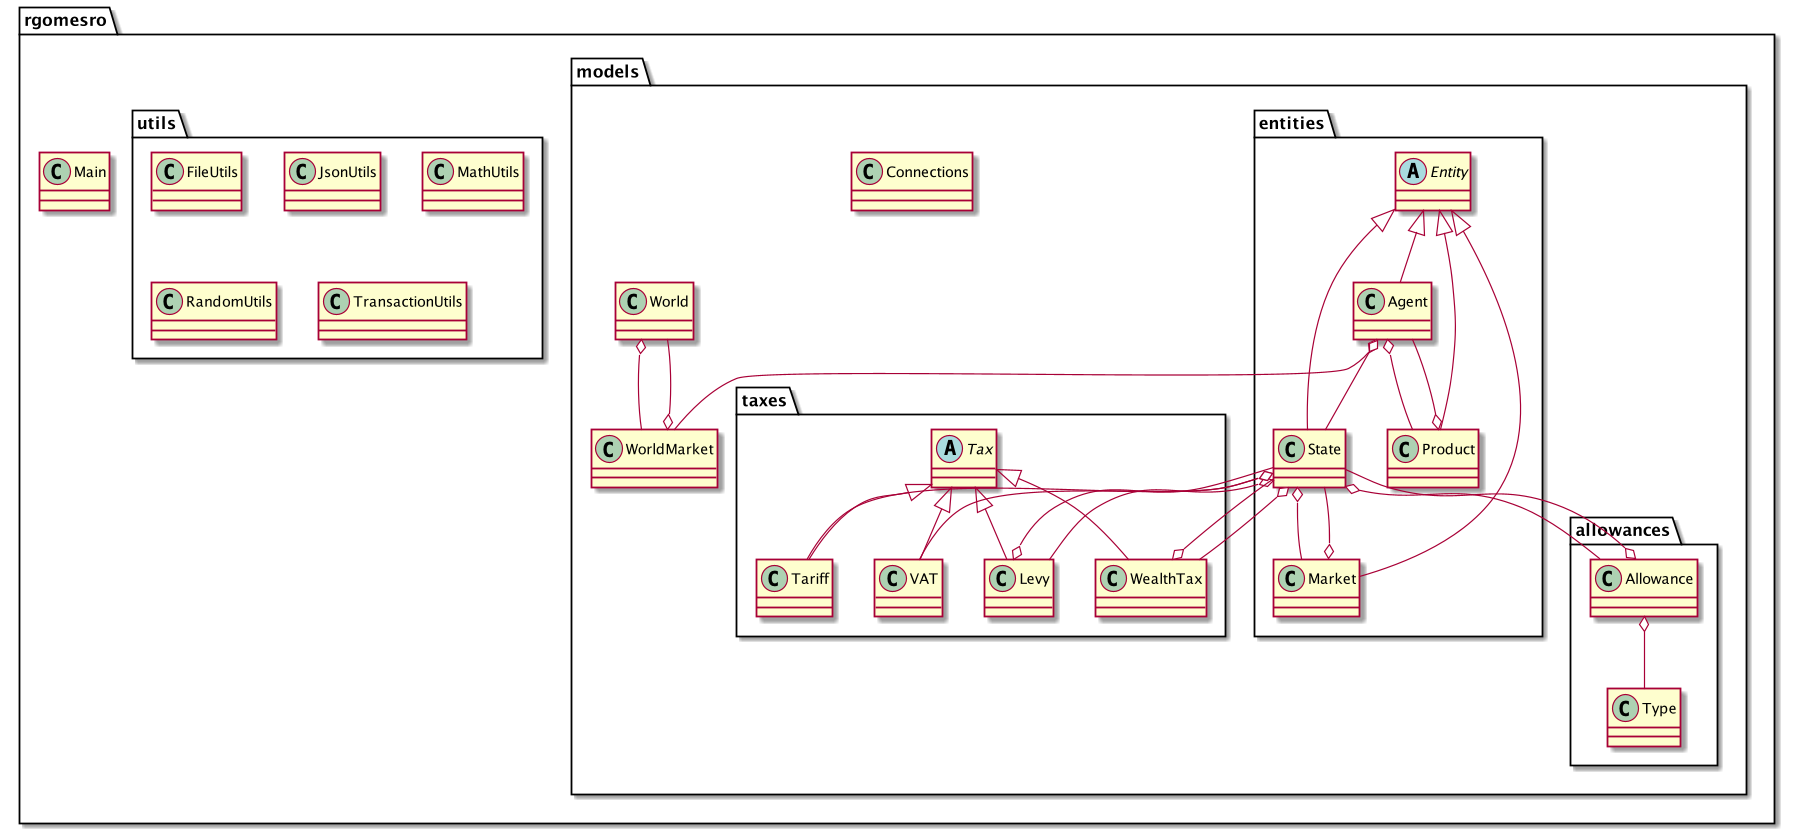
\includegraphics[width=1\textwidth]{img/generalCD.png}
        \caption{General class diagram}
        \label{fig:class_diagram_general}
    \end{figure}


    \begin{figure}[H]
        \centering
        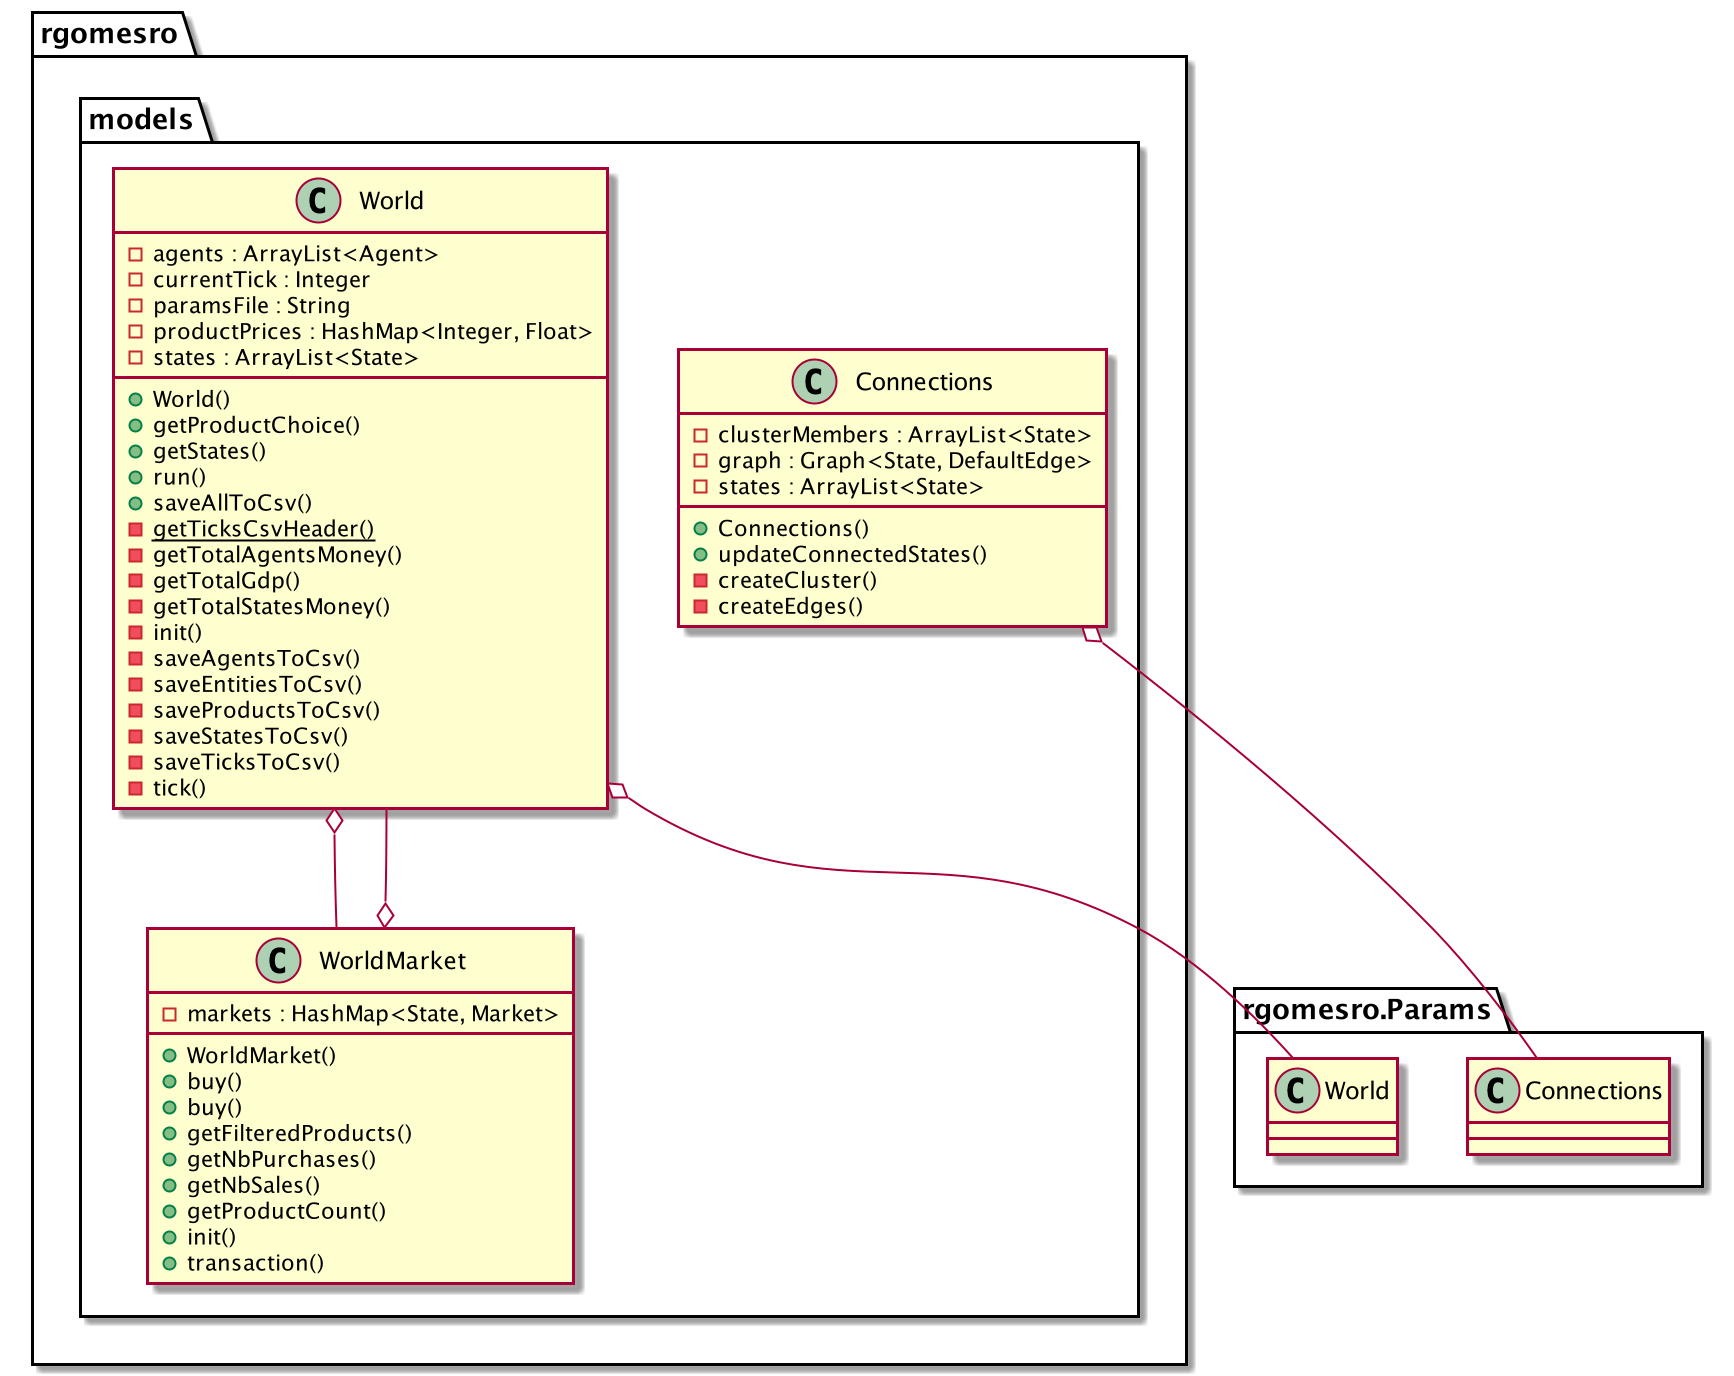
\includegraphics[width=1\textwidth]{img/modelsCD.png}
        \caption{Models class diagram (World, World Market and Connections)}
        \label{fig:class_diagram_models}
    \end{figure}


    \begin{figure}[H]
        \centering
        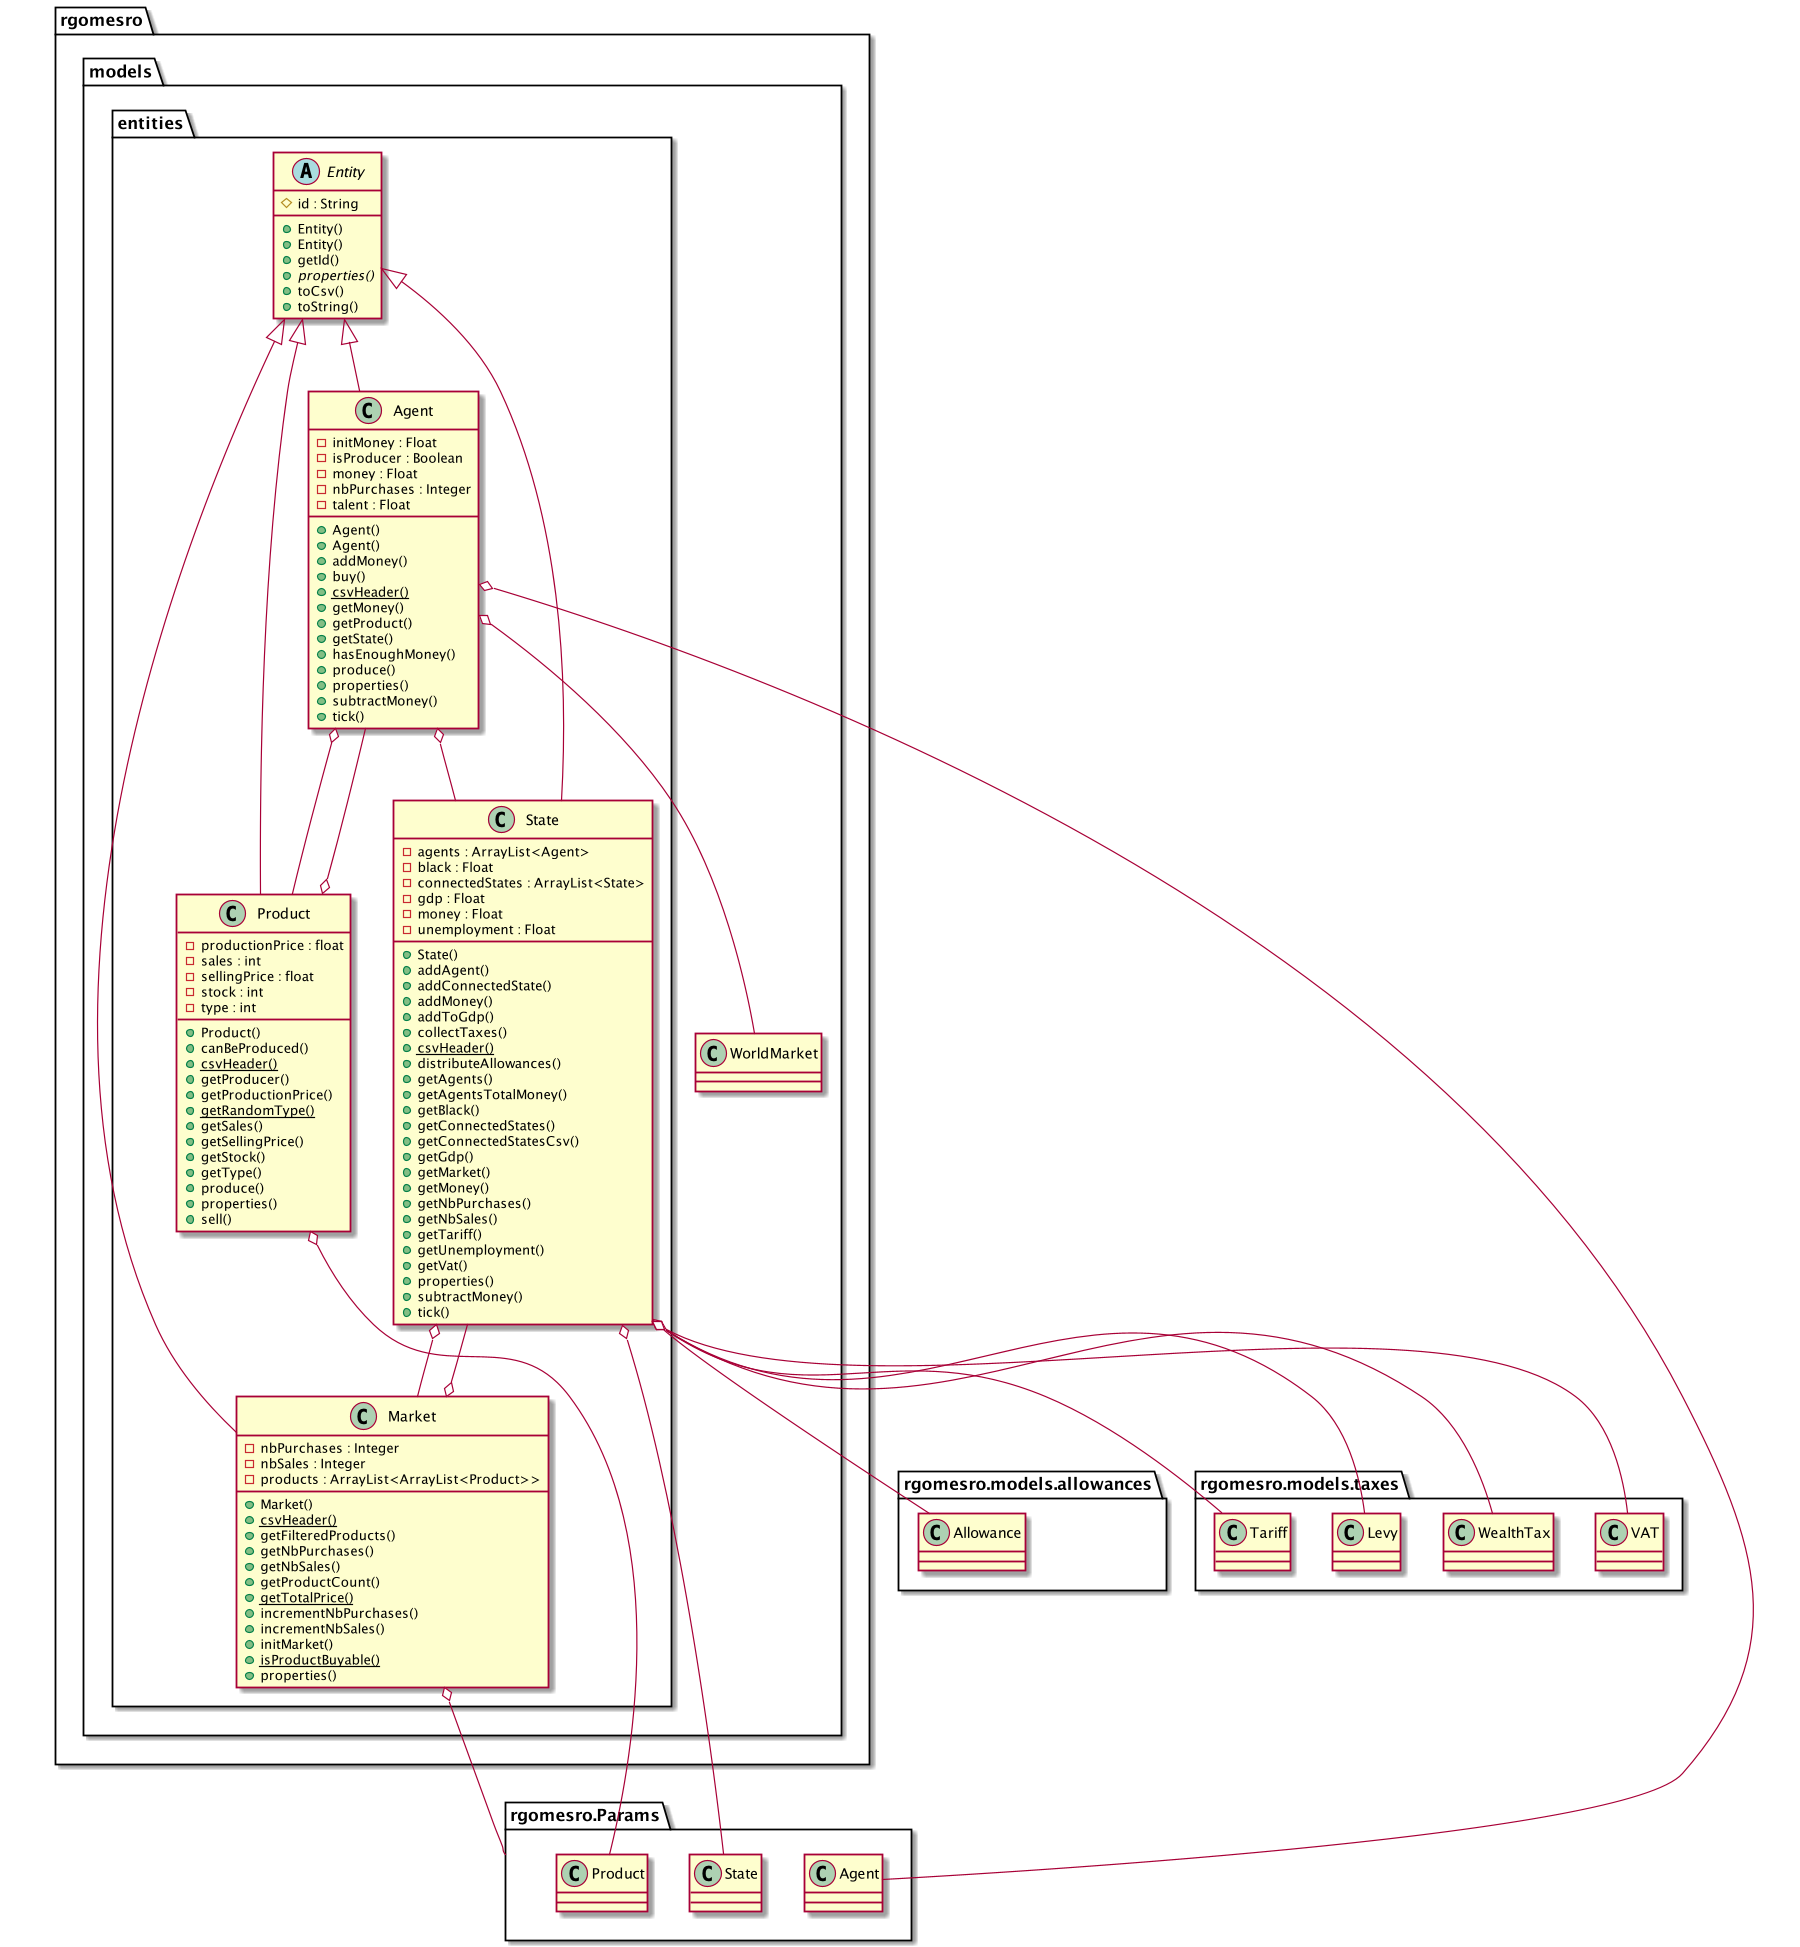
\includegraphics[width=1\textwidth]{img/entitiesCD.png}
        \caption{Entities class diagram (Agent, State, Product, Market)}
        \label{fig:class_diagram_entities}
    \end{figure}


    \begin{figure}[H]
        \centering
        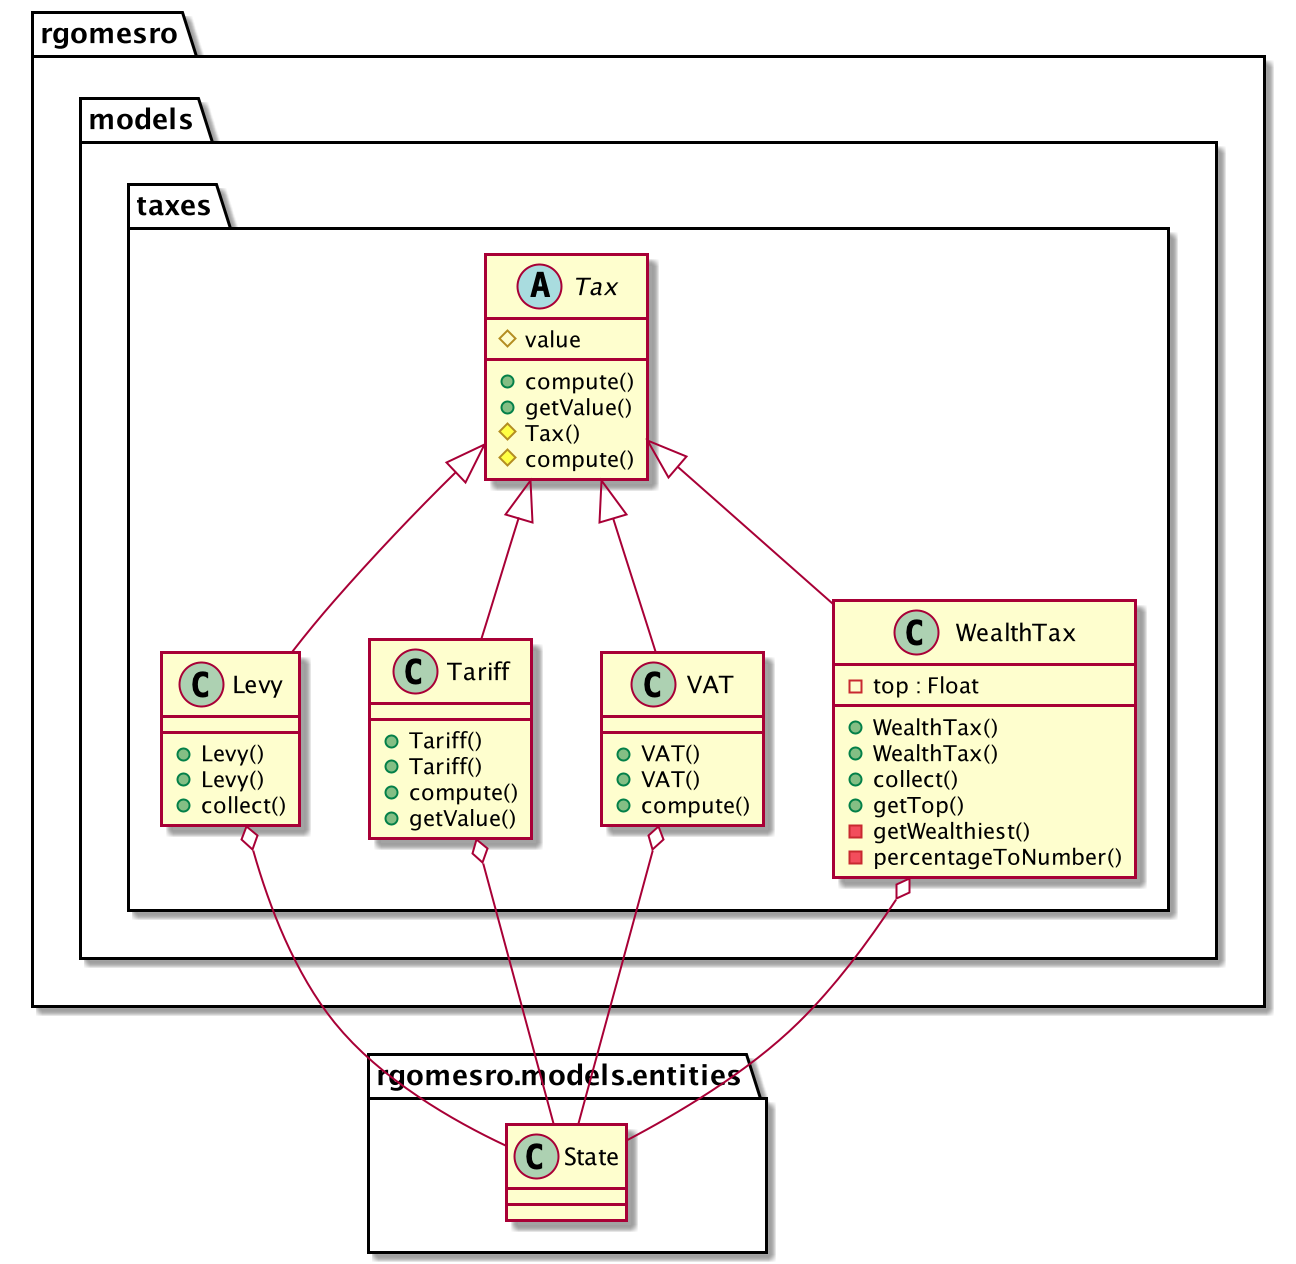
\includegraphics[width=0.7\textwidth]{img/taxesCD.png}
        \caption{Taxes class diagram (VAT, Levy, WealthTax, Tariff)}
        \label{fig:class_diagram_taxes}
    \end{figure}


    \begin{figure}[H]
        \centering
        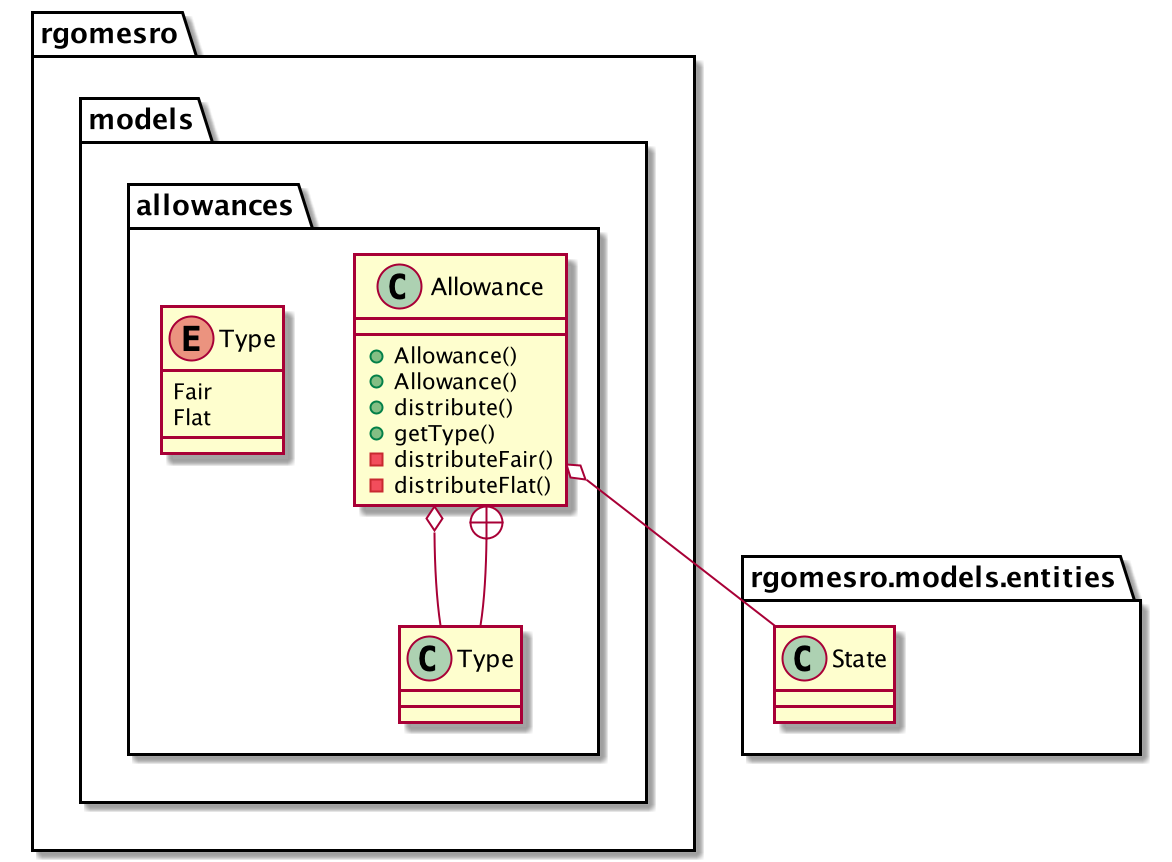
\includegraphics[width=0.7\textwidth]{img/allowancesCD.png}
        \caption{Allowances class diagram}
        \label{fig:class_diagram_allowances}
    \end{figure}


\chapter{Experiments}


\section{Introduction}

As we have seen in the previous section, all results of a simulation are stored into several \texttt{.csv} files.

\begin{itemize}
    \item \texttt{states.csv} contains, for each State, its id, population size, VAT rate, levy rate, tariff rate, wealth tax rate, allowance type, unemployment rate, black economy share, GDP, the money it has, the total money of its population (agents), the number of transactions performed by its agents, and the id's of the other States to which it is connected.

    \item \texttt{agents.csv} contains, for each Agent, its id, the id of its State, its initial money (the money with each it started the simulation), its current money, its talent, whether it is a producer or not (thus whether it is employed or unemployed) and the number of purchases it has made.
    
    \item \texttt{products.csv} contains, for each Agent, the id of the Agent producing it, its type, the production price (always set to 0), the selling price, the stock of this product, and the number of sales. Therefore, each agent has one Product and we can merge this file with the agents file.
    
    \item \texttt{ticks.csv} keeps track of different values during the simulation. The following metrics are saved every 100 ticks: the number of ticks that have passed so far, the number of transactions that have happened in the World so far, the total money of all the States, the total money of all the Agents, and the total GDP of all States.
\end{itemize}

Based on these files, we can do various experiments by adjusting the parameters and see the effects on some key metrics. For this, the language Python3 has been chosen as it contains many libraries to analyze and plot such data: pandas, numpy or matplotlib. Rapidness is not the key factor here as the simulation has already stored its results in the \texttt{.csv} files.

The default configuration file that we use is the following. Experiment after experiment, we will modify one or several parameter and see its/their influence. 

\begin{lstlisting}[language=json,firstnumber=1]
{
    "World": {
        "PRODUCT_CHOICE": "CHEAPEST",
        "NB_STATES": 500,
        "NB_AGENTS": 25000,
        "NB_TICKS": 3000,
        "NB_TICKS_SAVE_CSV": 100
    },
    "Connections": {
        "CLUSTER_SIZE": 0,
        "PROB_CONNECTION": 0.0
    },
    "State": {
        "Tax": {
            "MIN_VAT": 0.2,
            "MAX_VAT": 0.2,
            "MIN_LEVY": 0.1,
            "MAX_LEVY": 0.1,
            "MIN_TARIFF": 0.3,
            "MAX_TARIFF": 0.3,
            "VAL_WEALTH_TAX_TOP": 0.1,
            "MIN_WEALTH_TAX_VALUE": 0.2,
            "MAX_WEALTH_TAX_VALUE": 0.2,
            "NB_TICKS_COLLECT_TAXES": 100
        },
        "Allowance": {
            "NB_TICKS_DISTRIBUTE_ALLOWANCES": 100
        },
        "Others": {
            "MIN_UNEMPLOYMENT": 0.05,
            "MAX_UNEMPLOYMENT": 0.05,
            "MIN_BLACK": 0.15,
            "MAX_BLACK": 0.15
        }
    },
    "Agent": {
        "MIN_INIT_MONEY": 1000.0,
        "MAX_INIT_MONEY": 1000.0,
        "RATIO_BUY": 0.5,
        "RATIO_PRODUCE": 0.5
    },
    "Product": {
        "NB_DIFF_PRODUCTS": 50,
        "MIN_PRICE": 0.0,
        "MAX_PRICE": 300.0,
        "MAX_STOCK": 2000
    }
}
\end{lstlisting}

Whenever points are scattered on a plot, we will also plot a line which interpolates, with a degree 2, these points to better highlight the trend. Also, in the bar charts, an average is computed in order to give a global overview. We also have to pay attention that most plots have two $y$ axis (red is for the left hand-side, blue for the right hand-side). There are over 40 plots in the folder \texttt{./report/img/exp/}, we will only focus on the most interesting ones.

For each experiment, we will compare it with the state-of-the-art presented earlier, and try to answers the many research questions introduced in the section~\ref{section:motivation_objectives}.


\section{State experiments}

We will start our experiments with all the parameters related to the State. We should note that to be able to compare fairly different States, the metrics of the State (for instance the total money of its Agents or the GDP) is divided by its population size. 

    \subsection{Experiment 1: No taxes}
    In this first experiment, we will try to see the effects on having no taxes (thus all tax values are set to 0). In the following plots, we will plot the State with regular taxes (as defined earlier) on the left hand-side, and the State with no taxes on the right hand-size. 

        \subsubsection{State GDP and number of transactions}

        We can see on the following plots that a State with no taxes (thus VAT of 0, but the other taxes are also set to 0) will generally have a smaller GDP and the number of transactions is also decreased compared to a State with taxes (left plot where the VAT is 0.2 for instance). 
        
        At first this might seem rather odd since we expect products to be cheaper, therefore more transactions should be happening (hence the GDP would be boosted too). However, if we think more about it, this seems rather logical because a State with no tax will not be able to distribute allowances, and thus some agents will concentrate all the money at the expense of other agents who will not be able to buy products anymore after some time, eventually diminishing both the GDP and the number of transactions.

        \begin{figure}[H]
            \minipage{0.5\textwidth}
                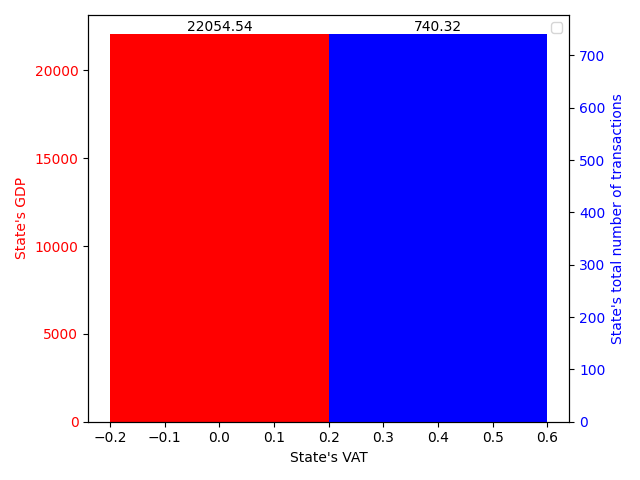
\includegraphics[width=\linewidth]{img/exp/1_1_1.png}
                \caption{Normal taxes (e.g. VAT of 0.2)}
            \endminipage\hfill
            \minipage{0.5\textwidth}
                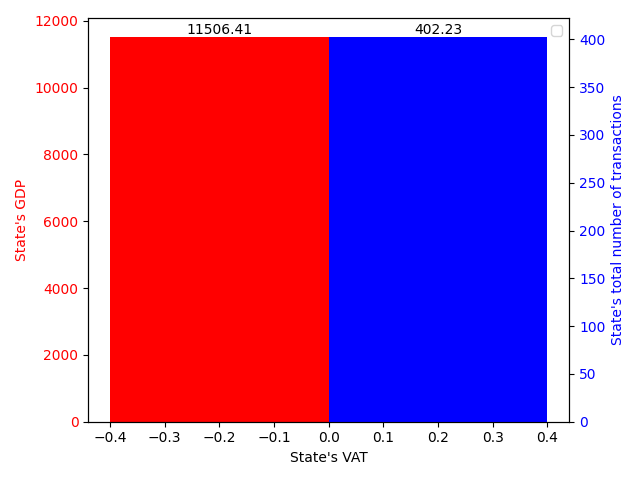
\includegraphics[width=\linewidth]{img/exp/1_2_1.png}
                \caption{No taxes (e.g. VAT of 0)}
            \endminipage\hfill
        \end{figure}

        \subsubsection{Gini coefficient} 
        
        Another interesting metric is the measure of inequalities, i.e. the Gini coefficient, the smaller it is, the more equal a society is. We can, naturally, see a tremendous difference between the two plots. Indeed, if the State has no taxes, it cannot collect nor distribute money. Therefore, the Gini coefficient skyrockets from $0.39$ to $0.96$.

        \begin{figure}[H]
            \minipage{0.5\textwidth}
                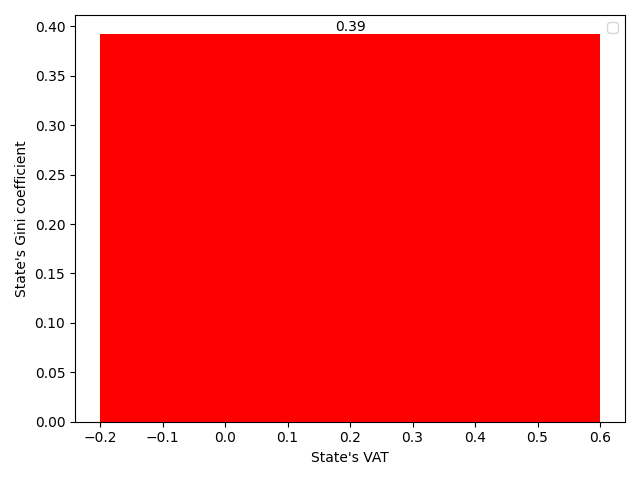
\includegraphics[width=\linewidth]{img/exp/1_1_3.png}
                \caption{Normal taxes (e.g. VAT of 0.2)}
            \endminipage\hfill
            \minipage{0.5\textwidth}
                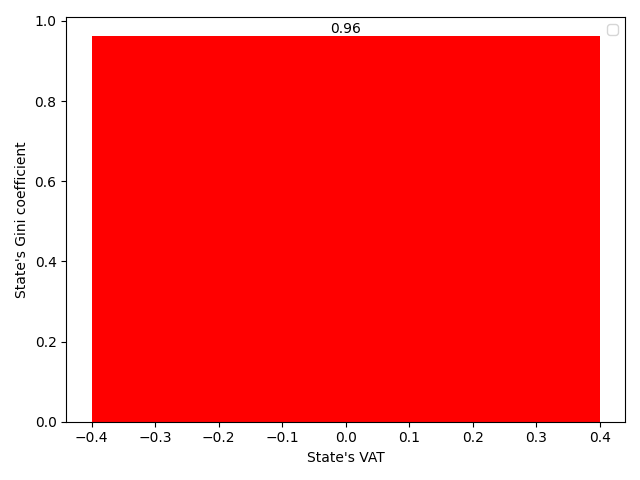
\includegraphics[width=\linewidth]{img/exp/1_2_3.png}
                \caption{No taxes (e.g. VAT of 0)}
            \endminipage\hfill
        \end{figure}

        This experiment shows the importance of having taxes (in the broadest sense of the term) on several metrics in order for our society to advance and be more fair.

    \subsection{Experiment 2: VAT}\label{section:expVAT}
    We will now, for each of the four taxes that were presented, analyze their influence. First: the VAT. For this, we will generate many States with random values for the VAT (ranging from 0 to 1) and see if we can see any pattern emerging regarding some metrics.

        \subsubsection{State GDP and number of transactions}

        \begin{wrapfigure}{l}{0.5\linewidth}
            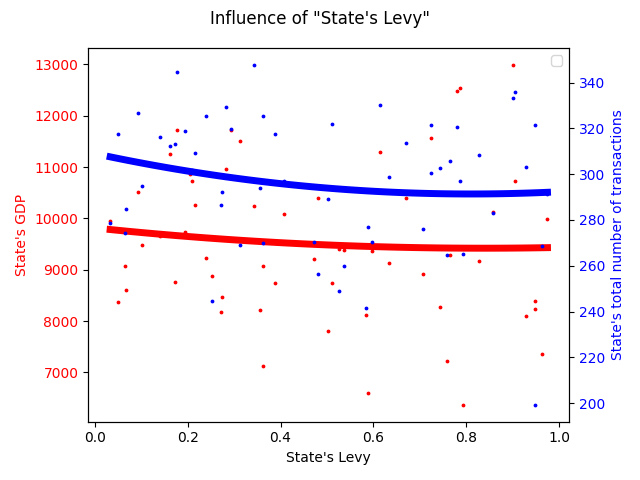
\includegraphics[width=\linewidth]{img/exp/2_1.png}
        \end{wrapfigure} 
        { At first, it is quite surprising to obtain such a plot where no correlation or pattern can be observed. Nonetheless, this makes sense because no matter what the VAT level is, agents will always be able to buy the same amount of products since the money collected from the taxes is always redistributed. For instance, if we have a VAT of 0, our agents will still be able to buy products because States have other taxes to collect money that they will redistribute afterwards. On the other side, if we have a VAT of 1, the State will have more money to redistribute, therefore agents will be richer. They could potentially buy more products, however this will not be the case because of such a high VAT rate making products more expensive.
        \par

        \subsubsection{Gini coefficient}

        \begin{wrapfigure}{r}{0.5\linewidth}
            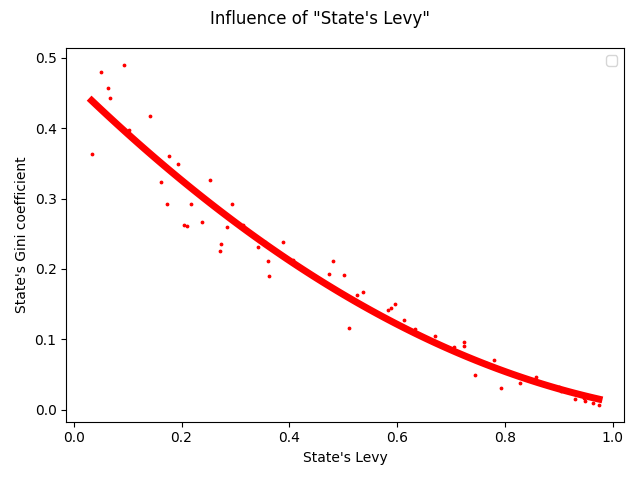
\includegraphics[width=\linewidth]{img/exp/2_3.png}
        \end{wrapfigure} 
        { \lipsum[1-2] Naturally, as we had seen before, the lower the VAT is, the more inequalities we will have since the State has less money to redistribute fairly. However, we can see that here, with a VAT of 0, the Gini coefficient is around 0.45 whereas it was at 0.91 before. This is because in this case, the other taxes are still present as shown in the default configuration allowing the State to distribute allowances and diminishing inequalities. Hence why the higher the VAT is, the less inequalities we have since the Gini coefficient tends to go to zero.
        \par

    \subsection{Experiment 3: Tariff}
    As for the VAT, we will now analyze the influence of the tariff tax by generating many States with random values (ranging from 0 to 1) and see if we can see any pattern emerging regarding some metrics. 

        \begin{figure}[H]
            \minipage{0.5\textwidth}
                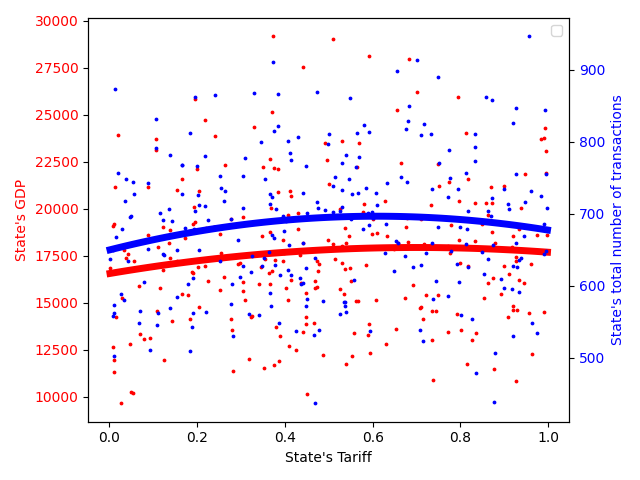
\includegraphics[width=\linewidth]{img/exp/3_1.png}
                \caption{State GDP and number of transactions}
            \endminipage\hfill
            \minipage{0.5\textwidth}
                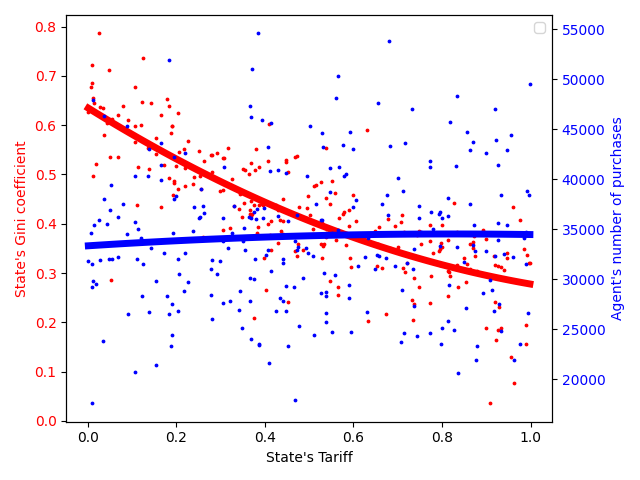
\includegraphics[width=\linewidth]{img/exp/3_3.png}
                \caption{Gini coefficient}
            \endminipage\hfill
        \end{figure}

        As for the previous experiment, the first plot might seem astonishing at first, but the explanation is exactly the same as for the previous experiment~\ref{section:expVAT}. The same goes for the second plot and the analysis of the Gini coefficient.


    \subsection{Experiment 4: Levy}\label{exp:levy}
    We will now analyze the influence of the levy tax by generating many States with random values (ranging from 0 to 1) and see if we can see any pattern emerging regarding some metrics. 

        \begin{figure}[H]
            \minipage{0.5\textwidth}
                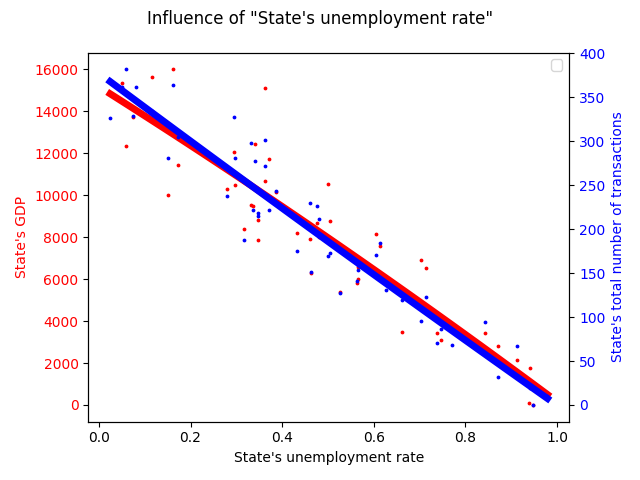
\includegraphics[width=\linewidth]{img/exp/4_1.png}
                \caption{State GDP and number of transactions}
            \endminipage\hfill
            \minipage{0.5\textwidth}
                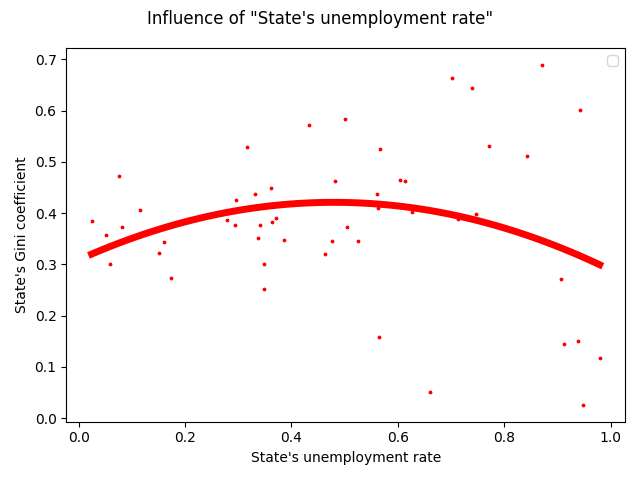
\includegraphics[width=\linewidth]{img/exp/4_3.png}
                \caption{Gini coefficient}
            \endminipage\hfill
        \end{figure}

        As for the previous experiments, the first plot might seem astonishing at first, but the explanation is exactly the same as for the previous experiment~\ref{section:expVAT}. The same goes for the second plot and the analysis of the Gini coefficient. However, in this experiment, the Gini coefficient goes down until almost zero. This was to be expected because if we levy 100\% of the wealth of all agents, they will be moneyless. Therefore, after redistributing the allowances, they will all have the money. Indeed, the Fair and Flat allowance will be almost exactly the same since all agents have the same wealth: none.

    \subsection{Experiment 5: Wealth tax}
    We will now analyze the influence of the last tax: the wealth tax with the same methodologies as the previous taxes and see if we can see any pattern emerging regarding some metrics. 

        \begin{figure}[H]
            \minipage{0.5\textwidth}
                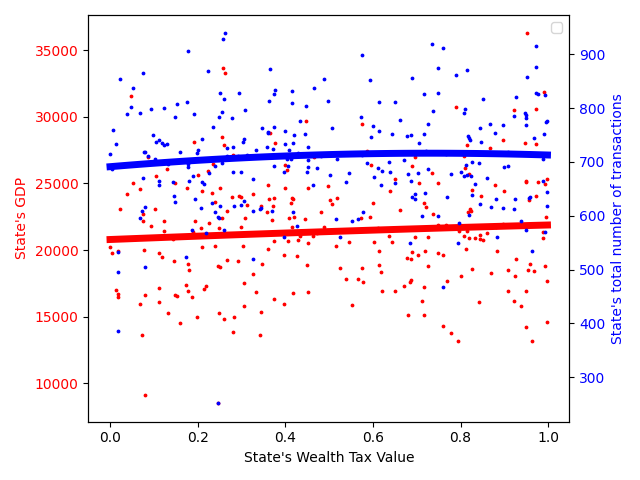
\includegraphics[width=\linewidth]{img/exp/5_1.png}
                \caption{State GDP and number of transactions}
            \endminipage\hfill
            \minipage{0.5\textwidth}
                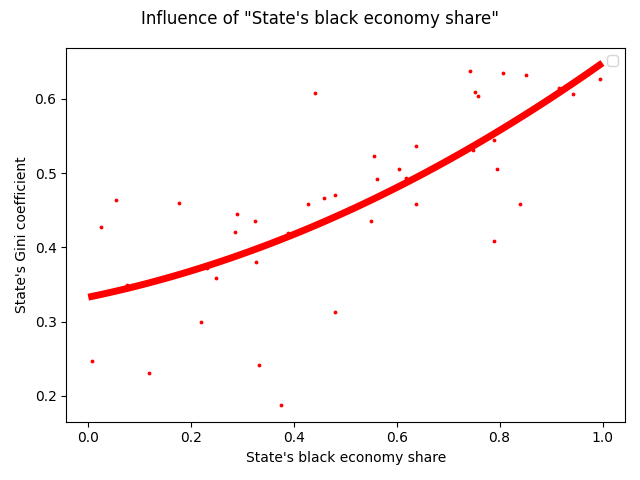
\includegraphics[width=\linewidth]{img/exp/5_3.png}
                \caption{Gini coefficient}
            \endminipage\hfill
        \end{figure}

        As for the previous experiments, the first plot might seem astonishing at first, but the explanation is exactly the same as for the previous experiment~\ref{section:expVAT}. The same goes for the second plot and the analysis of the Gini coefficient.


    \subsection{Experiment 6: Unemployment}\label{exp:unemployment}
    After analyzing the different taxes, we will now focus on another parameter which cannot directly be controlled by the State. As usual, we will create many States with different unemployment rates and see how our metrics change.

            
        \subsubsection{State GDP and number of transactions}

        \begin{wrapfigure}{l}{0.5\linewidth}
            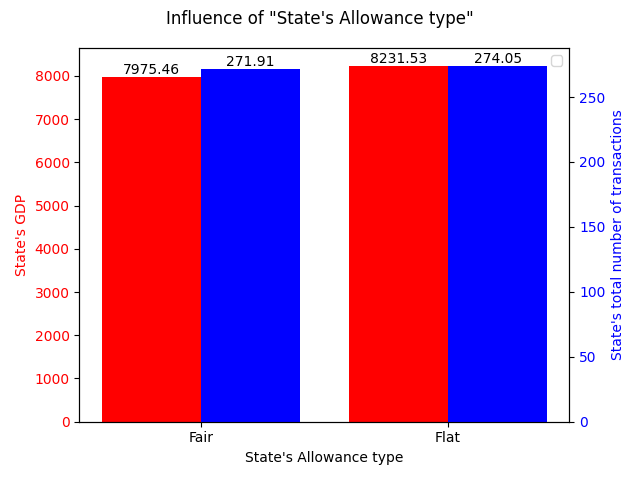
\includegraphics[width=\linewidth]{img/exp/6_1.png}
        \end{wrapfigure} 
        {As one could have expected, we have a rather clear linear correlation. Indeed, the higher the unemployment rate is, the less number of transactions we have and the lower the GDP is. Actually, it is a vicious cycle because the less producers we have, the less products are available on the market, thus less transactions. By having less transactions, we collect less taxes, and therefore do not distribute as much, this means that some agents will never be able to buy another product. 
        \par

        \subsubsection{Gini coefficient}

        \begin{wrapfigure}{r}{0.5\linewidth}
            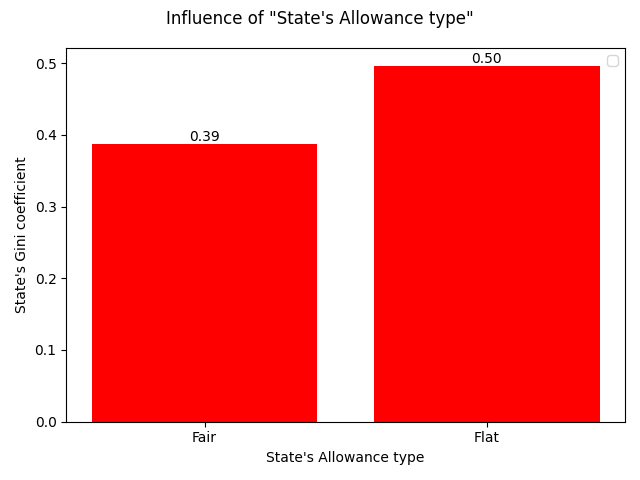
\includegraphics[width=\linewidth]{img/exp/6_3.png}
        \end{wrapfigure} 
        {The plot on the side is a bit tricky but more interesting to analyze. If we only look at the scattered points, we see that there is a linear correlation from the rate 0.0 until 0.8: the more non-producing agents we have, the bigger the Gini coefficient is. This is logical because producing agents will still be able to sell their products and make some money thus accumulating more wealth compared to others, increasing the inequalities.

        However, after the 0.8 rate on the $x$ axis, we can see a significant drop, and the previous statement does not hold true anymore: the Gini coefficient gets very close to zero, i.e. perfect equality. Actually, it also makes sense because if almost everybody is unemployed, then no one can afford to buy any product, thus we have almost no transactions happening and no money flowing between agents, and no agent can therefore become richer than others.
        \par


    \subsection{Experiment 7: Black economy}\label{exp:black}
    The second parameter which cannot directly be controlled by the State is the black economy. As usual, we will create many States with different share of black economy happening and see how our metrics change.

            
        \subsubsection{State GDP and number of transactions}

        \begin{wrapfigure}{l}{0.5\linewidth}
            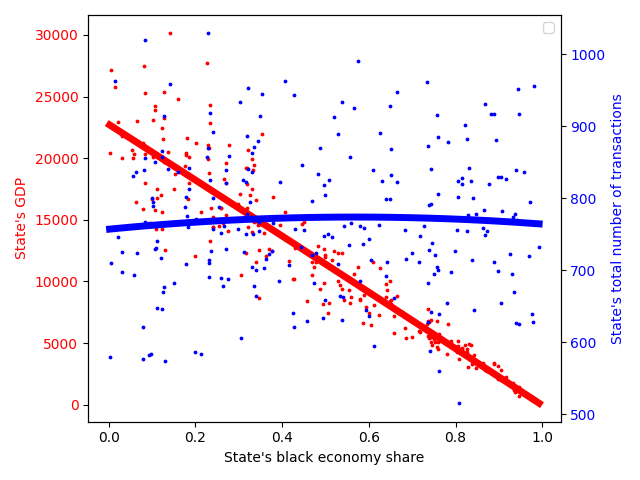
\includegraphics[width=\linewidth]{img/exp/7_1.png}
        \end{wrapfigure} 
        {Until now, we were used to see a strong relation between the number of transactions and the State's GDP. However, this is not the case anymore because of the black economy (because even when no due tax is paid, the transaction is still counted). This results in a linear correlation between the black economy share and the GDP as expected, yet we see absolutely no correlation with the number of transactions since the blue line is quite straight.
        \par

        \subsubsection{Gini coefficient}

        \begin{wrapfigure}{r}{0.5\linewidth}
            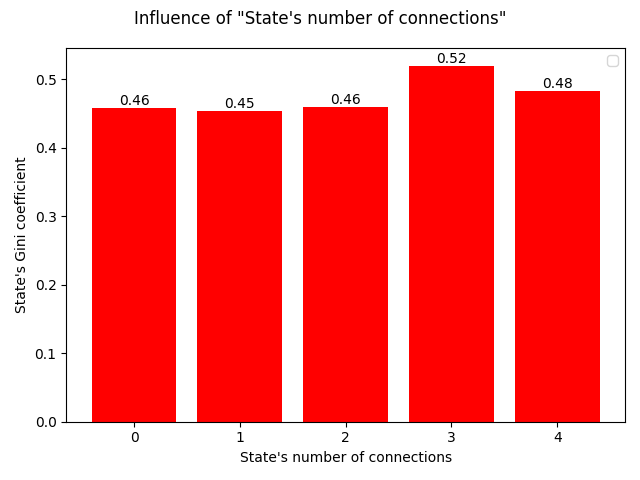
\includegraphics[width=\linewidth]{img/exp/7_3.png}
        \end{wrapfigure} 
        {As the black economy share increases, the inequalities augment as well. This is simply due to the fact that the State will have less money to redistribute when giving allowances, therefore inequalities will subsist even after the small amount of money collected as been redistributed. \\ \\
        \par
    


    \subsection{Experiment 8: Allowances}\label{exp:allowances}
    As we have seen, we have two types of allowances: the flat one (which mimics the Universal Basic Income in the sense that the money is distributed regardless of the agent's wealth), and the fair one (based on the agent's wealth). We will analyze the effects of these two types of redistribution mechanisms.
    
        \subsubsection{State GDP and number of transactions}

        \begin{wrapfigure}{l}{0.5\linewidth}
            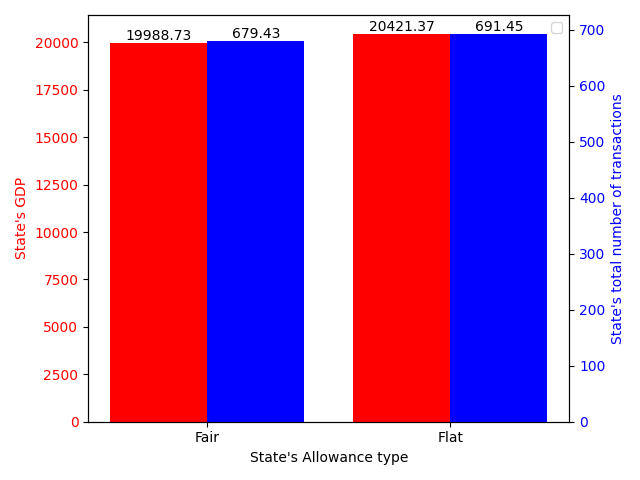
\includegraphics[width=\linewidth]{img/exp/8_1.png}
        \end{wrapfigure} 
        { On this side plot, we see that the flat redistribution mechanism seems to be \emph{slightly} superior to the fair one. The increase is of about $2\%$ (2.1\% for the GDP going from $19988$ to $20421$ and $1.7\%$ for the number of transactions going from 679 to 691). This increase is rather negligible and might be the result of the stochastic behavior of the simulation. Indeed, one would expect to not be a relevant difference on these metrics. For instance, the number of transactions is not penalized by the Flat allowance because poorer agents will still be able to afford buying products since they receive their (equal) share of the total money distributed: all Agents are still able to buy products,.
        \par

        \subsubsection{Gini coefficient}

        \begin{wrapfigure}{r}{0.5\linewidth}
            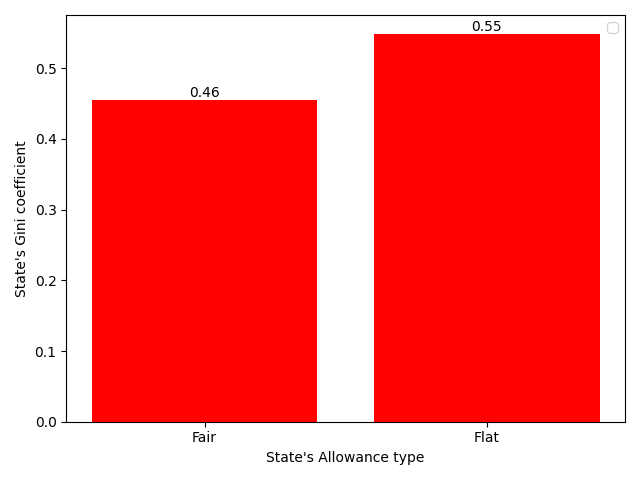
\includegraphics[width=\linewidth]{img/exp/8_3.png}
        \end{wrapfigure} 
        { On the contrary, one would expect a quite pertinent difference on the metric of inequalities as depicted on the plot. This results seems logical since it is was the \emph{main goal} of this redistribution system: State distributing the collected money in a fair way have, in average, a smaller Gini index (i.e. inequalities are limited) and vice-versa for the flat distribution mechanism. With this flat allowance, the wealthier agents will stay wealthier.

        However, an important note to make is that both these systems clearly outperform the system where no redistribution is in place. Indeed, we had seen in the first experiment that, in this case, the Gini coefficient would skyrocket to $0.96$.
        \par



    \subsection{Experiment 9: Connections}
    The final parameter of States that will be analyzed is the number of Connections it has. For this we will study both the bilateral connections and the cluster and their influence on our already well presented metrics. In this experiment, we have a probability of connection of 0.3 and a cluster of 5 States (thus each State is connected to 4 others).

        \subsubsection{State GDP and number of transactions}

        \begin{wrapfigure}{l}{0.5\linewidth}
            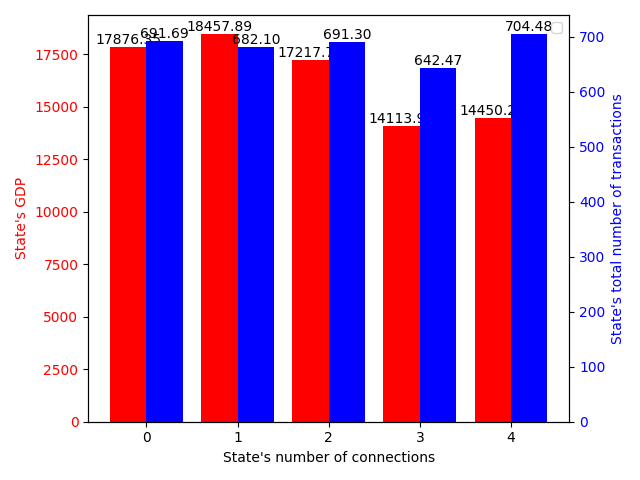
\includegraphics[width=\linewidth]{img/exp/9_1.png}
        \end{wrapfigure} 
        { First, as the number of connected states increases, it seems that the average GDP of these states decreases. Although this may seem odd at first, it fits with our implementation because agents will tend to buy cheaper products since they have a wider range of choices. On the other side, the number of transactions remains quite constant (besides the small drop when a State is connected to 3 others which might be due to the fact that not many States have 3 connections and therefore the statistical relevance is biased).

        With these metrics going towards opposite directions, we can notice something very interesting: the difference between the red (GDP) and blue (number of transactions) bars keeps increasing. Indeed, at first, when a State is connected to no other State, these two metrics are very related as we have seen up until now (besides in the black economy experiment). However, the difference is much more noticeable when a State is connected to 4 other States. The main hypothesis for this behavior is that agents perform as many transactions as before, however because they have access to other markets without any tariffs, they are able to buy some products at a cheaper price in another State therefore not increasing the GDP as much.

        The results of this experiment are quite lackluster when compared to the state of the art. Indeed, an increase of the GDP was expected for State with more connections. This difference is due to the code implementation which does not mimic well enough the reality, and not to the simulation itself. The simulation results fit the implementation.
        \par

        \subsubsection{Gini coefficient}

        \begin{wrapfigure}{r}{0.5\linewidth}
            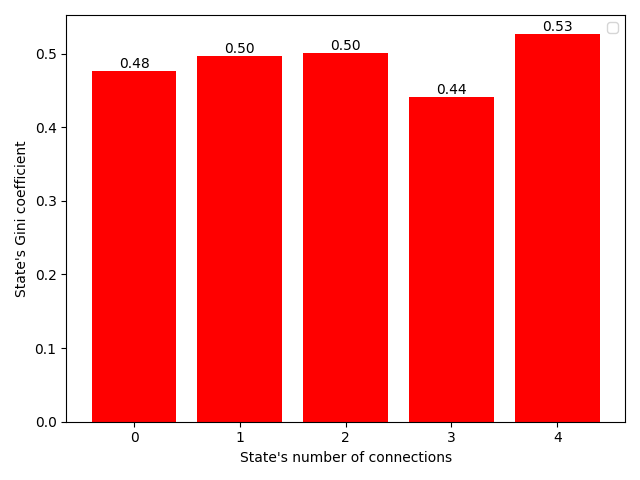
\includegraphics[width=\linewidth]{img/exp/9_3.png} 
        \end{wrapfigure}   
        { Regarding the measure of inequalities, we see that all the Gini coefficients are very similar to one another. The differences are quite negligible when compared to the others when had before (0.46 versus 0.55, or 0.39 versus 0.96). Having access to a larger market with cheaper prices does not, in fine, mean that inequalities will be reduced/accentuated for those agents since both the wealthiest and the poorest agents will buy these cheaper products, therefore no reduction of difference of wealth was expected. 
        \par
    

    \subsection{Experiment 10: Number of ticks}
        
        \begin{wrapfigure}{l}{0.5\linewidth}
            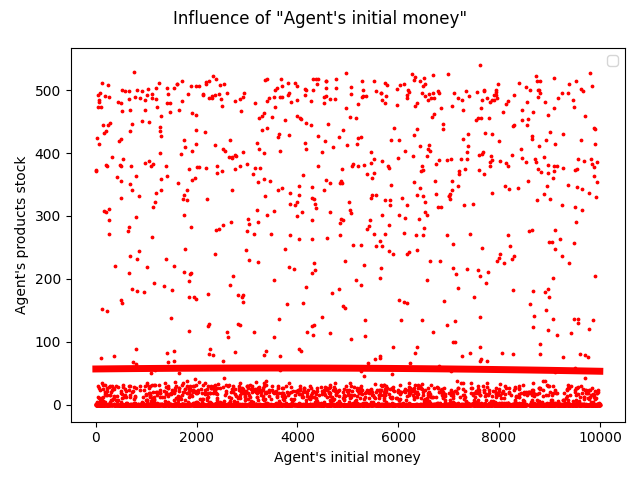
\includegraphics[width=\linewidth]{img/exp/10_2.png}
        \end{wrapfigure} 
        { Our last experiment of this section is not based on a parameter of the state \emph{per se}, but on the duration of the simulation and the evolution of some State metrics as the number of ticks increases. Deciding how long the simulation should run for is important to save computational power and run-time by checking at around how many ticks the simulation starts to stabilize. After this point of stabilization, there is no real advantage of running the simulation for even longer because no dramatic fluctuation should happen. 
            
        As we can see on this plot, the simulation metrics start to stabilize after 2000 or 3000 ticks and going up to 6000 ticks provides no advantage (for a run-time 2-3 times longer). Hence, the default number of ticks in the configuration file is 3000.
        \par
    
\section{Agent experiments}
    After seeing and analyzing some State parameters, we will focus on those of the Agents.

    \subsection{Experiment 11: Talent}
    The talent an agent has lets it produce cheaper products therefore having more chances at getting picked by a potential buyer looking for the cheapest product. For this experiment, we will analyze how the talent of an agent (between 0 and 1) influences its sales and purchases by generating lots of homogeneous agents with different talent values.

        \begin{wrapfigure}{r}{0.5\linewidth}
            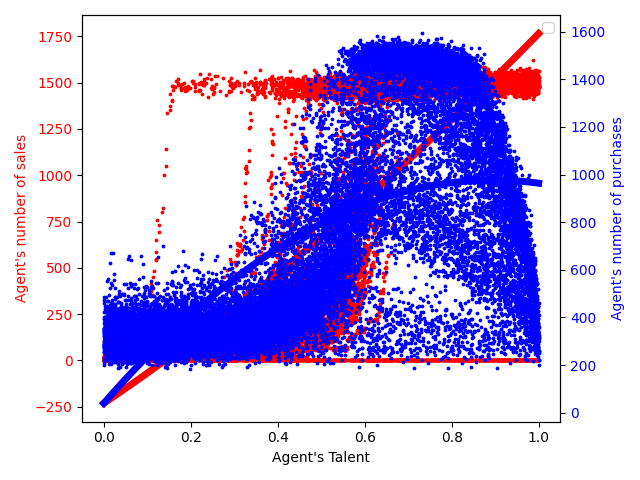
\includegraphics[width=\linewidth]{img/exp/11.png}
        \end{wrapfigure} 
        { This first plot may look quite chaotic and random at first, however we can see many interesting patterns by taking into account some particularities afterwards. First, generally we see a trend (red line behind the blue dots) that the more talent an agent has, the more sales it will make. Regarding the number of purchases, we have a rather odd pattern (which looks like the on in the Gini coefficient in the Unemployment experiment): as the talent increases, we are gradually able to make more purchases until a certain point around 0.5-0.7. After this point, there is a significant drop due to the fact that agents will produce products ``too cheap'', therefore not allowing them to earn enough wealth and make purchases. This is quite interesting because it shows that selling at such low prices is not always a good idea.
        
        However, it seems that the trends are not linear (as one could have expected) but this due to the fact a different products have different base prices (i.e. the original price of the product which is then lowered by a certain factor based on the agent's talent). For instance, if we have an agent A which produces a product with a base price of 10 with a talent of 0.1, then A will see its product at 9. Now if we have another agent B which produces a product with a base price of 200 with a talent of 0.7, its product will now cost 60. This means that, even though A has less talent (0.1) than B (0.7), it will \emph{probably} sell more products since its product remains cheaper, therefore we do not have a clear linear trend.
        This is also the reason why we a trace of red scattered points going upwards: the same product: the point goes up (i.e. more sales) as the talent goes up too.

        \par


    \subsection{Experiment 12: Initial money}
    Another interesting parameter is the initial money of an agent. Whether an agent starts the simulation with a small or huge amount of money could influence its purchases and sales. 

        \begin{wrapfigure}{l}{0.5\linewidth}
            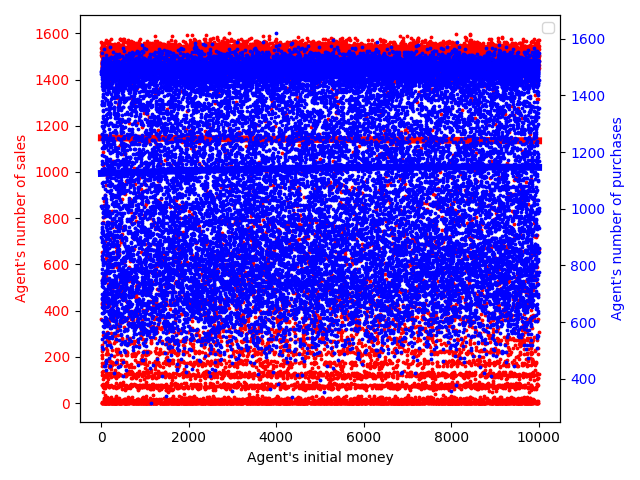
\includegraphics[width=\linewidth]{img/exp/12_1.png}
        \end{wrapfigure} 
        { Again, the plot looks a bit chaotic because of the many points (i.e. agents). However, we can clearly see that there is absolutely no correlation between the agent's initial money and its sales or purchases (both the blue and red lines are horizontal and the scattered points are very sparse across the plot). This was to be expected because of the redistribution. Indeed, although an agent may start with little money, it will still be able to make purchases with the money it receives from its sales and from the allowances it will receive during the simulation. 
        \par



    \subsection{Experiment 13: Unemployment}
    As we had seen in a previous experiment, unemployment (i.e. agent who never produces) plays a major role in the System. How can agents who do not produce make purchases ? For this experiment we will only have one State with a thousands agents and un employment rate of 0.3. To see the role of unemployment, we will compare one simulation which runs for 1000 ticks, and another for 10000 ticks.

        \begin{figure}[H]
            \minipage{0.5\textwidth}
                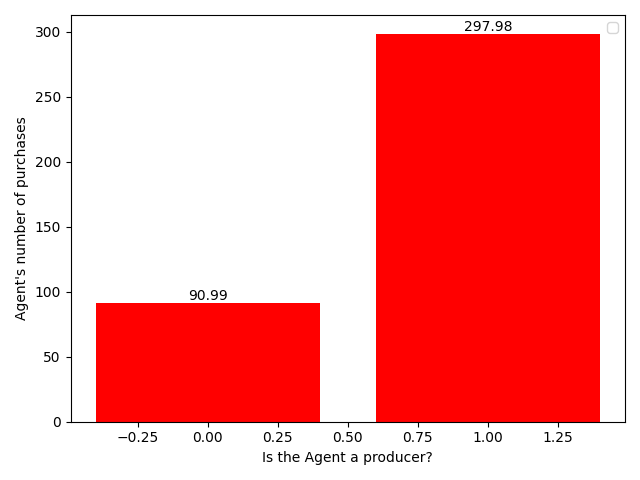
\includegraphics[width=\linewidth]{img/exp/13_1.png}
                \caption{1000 ticks}
            \endminipage\hfill
            \minipage{0.5\textwidth}
                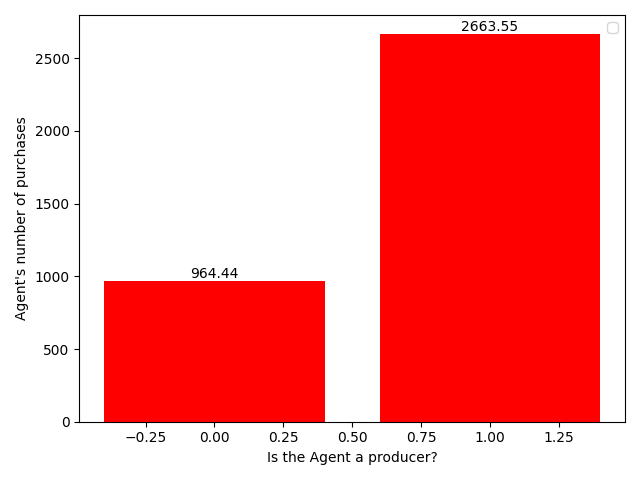
\includegraphics[width=\linewidth]{img/exp/13_2.png}
                \caption{10000 ticks}
            \endminipage\hfill
        \end{figure}

    As we can see on these plots (where 1 means that the agent is indeed a producer, and 0 means it is unemployed). Naturally, producers make more purchases than non-producers (2.2x times as much for 1000 ticks and 1.7x as much for 10000 ticks). However, we can see that in both cases, multiplying by 10 the number of ticks results in a \emph{roughly} 10 times increase of the number of purchases for both producers and non producers. This means that  non-producing agents can make purchases thanks to the redistribution system. Indeed, otherwise, if they were no allowances, the non-producing agents would be able to buy products up until a certain point where they have spent all their initial money. From that tick forward, they would not be able to make any purchase because they would not sell anything nor receive any money from the State, therefore a threshold would be reached, and increasing the number of ticks would not upgrade the threshold (contrary to here).
    

    \subsection{Experiment 14: Wealth distribution}
    We can see in the following comparison the difference between the wealth distribution among agents. This wealth distribution is presented by the Lorenz curve (in blue). 

    \begin{figure}[H]
        \minipage{0.5\textwidth}
            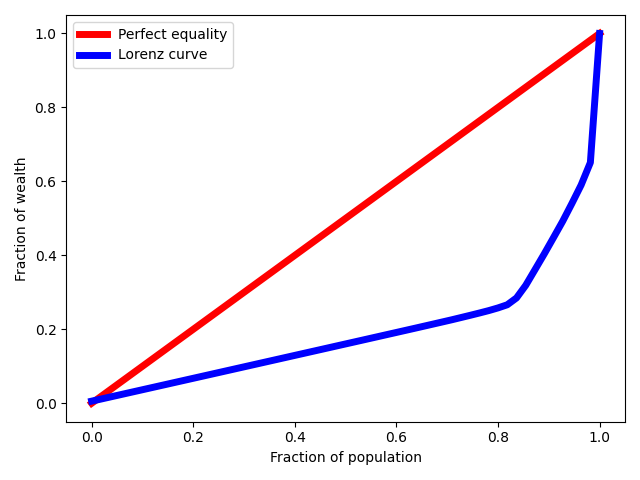
\includegraphics[width=\linewidth]{img/exp/14_1.png}
            \caption{Flat allowance State}
        \endminipage\hfill
        \minipage{0.5\textwidth}
            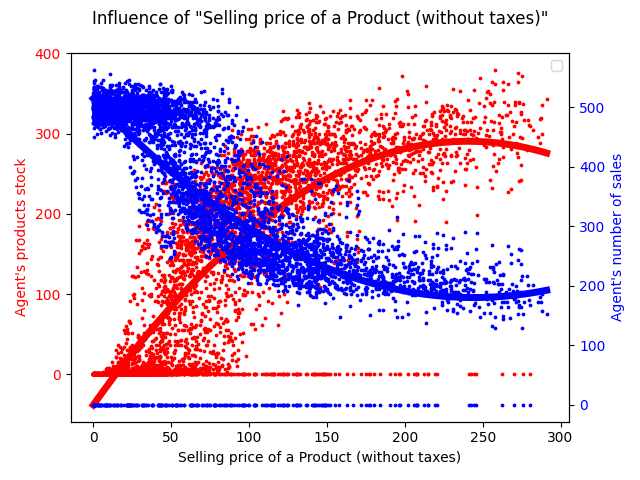
\includegraphics[width=\linewidth]{img/exp/14_2.png}
            \caption{Fair allowance State}
        \endminipage\hfill
    \end{figure}

    We can read this plot as follows: if we take the x point 0.8 in the left hand-side plot, we can see that 80\% of the population owns around 25\% of the total wealth. On the other plot, we see that at 80\% of the population owns around 40\% of the total wealth. Therefore, the second case seems fairer. In a perfect equality society, we would obtain the red curve: 30\% of the population detains 30\% of the wealth, 80\% would own 80\%, etc. 
    
    Therefore, the bigger the area between the red and blue curves, the higher the inequalities will be. This area actually represents one metric that we have analyzed all along this thesis: the Gini coefficient. If both curve coincide, the Gini index will be 0. On the other side, if there is only one person holding all the wealth and all the others agents own nothing, then we would see a blue horizontal line at the bottom with a sudden peak at then end therefore resulting in a Gini coefficient very close to 1. \footnote{Not \emph{exactly} 1 because we would need an infinite amount of agents}.

    The Gini coefficient on the left plot (where a flat allowance redistribution system is used) is equal to 0.618 whereas on the right hand-side the Gini index is equal to 0.546. Naturally, we can see that the right case is fairer as wealth is distributed a bit more fairly.


\section{Product experiments}
    Finally, our last two experiments will be about the products. 


    \subsection{Experiment 15: Selling price}
    

        \begin{wrapfigure}{l}{0.5\linewidth}
            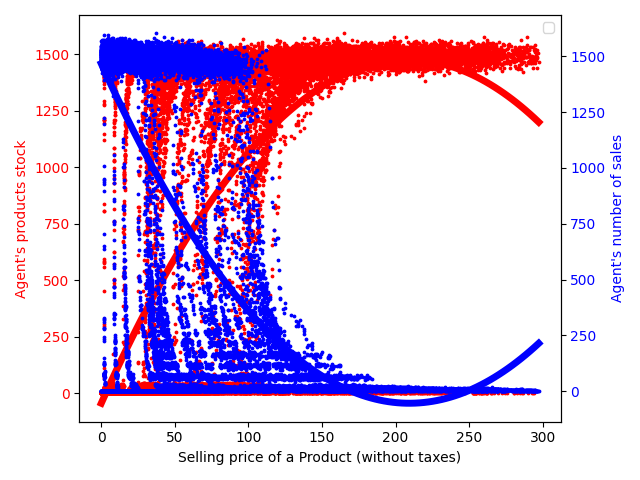
\includegraphics[width=\linewidth]{img/exp/15.png}
        \end{wrapfigure} 
        { The first basic parameter of a product is the selling price. We can analyze its impact on two metrics: the number of stocks remaining, and, of course, the number of sales of that product. Naturally, these two curves metrics are the opposite of each other: more sales means less stocks remaining. We see that the trends are not totally linear. This is because we are analyzing the selling price without any taxes. By adding the VAT and the custom tariffs (if applicable), a cheaper product might become more expensive, therefore resulting in these solitary scattered points. 
        \par


    \subsection{Experiment 16: Choosing method}
    As introduced before, after an agent filters the available products according to their type, price, etc., it should choose one among those possibilities. There are three ways of picking a product: cheapest, random, weighted-random as previously explained. We will analyze these three choosing methods.

    \begin{figure}[H]
        \minipage{0.32\textwidth}
            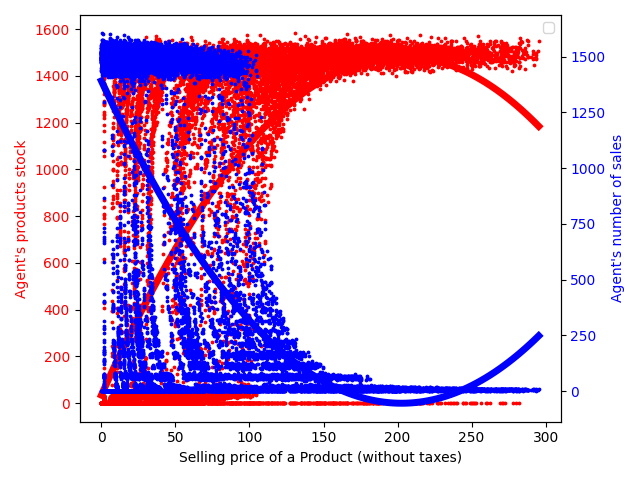
\includegraphics[width=\linewidth]{img/exp/16_1.png}\label{fig:cheapest}
            \caption{Cheapest}
        \endminipage\hfill
        \minipage{0.32\textwidth}
            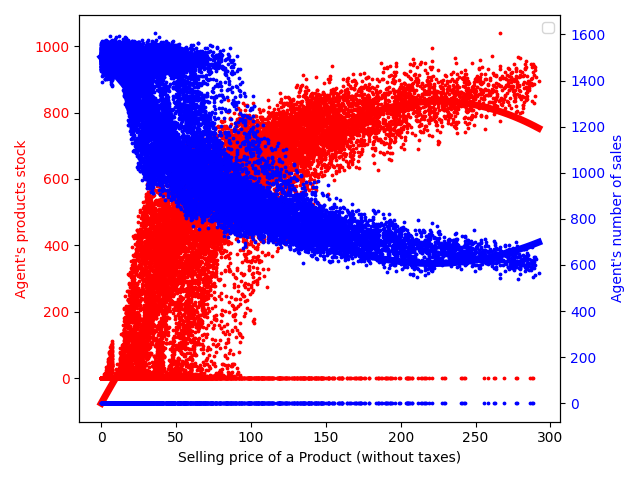
\includegraphics[width=\linewidth]{img/exp/16_2.png}\label{fig:random}
            \caption{Random}
        \endminipage\hfill
        \minipage{0.32\textwidth}
            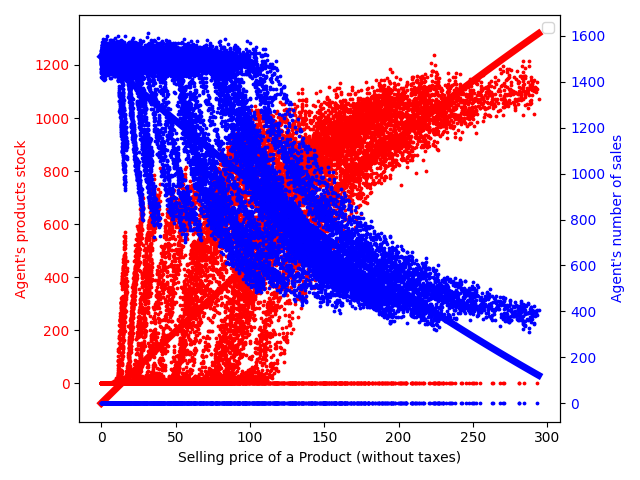
\includegraphics[width=\linewidth]{img/exp/16_3.png}\label{fig:weighted}
            \caption{Random weighted}
        \endminipage\hfill
    \end{figure}

    The first plot has already been analyzed and explained in the previous section (because the default choosing method is 'Cheapest'). We will compare it with other two methods. 
    
    In the middle plot, where a random method is used, we can see that agents will more easily buy more expensive products since we have more scattered points on the right hand-side of the plot (compared to the first plot) as we wanted. Although products are selected at random despite the price, we must recall that we have a filtered list of \emph{possibilities} according to the budget of the agent. Thus, naturally, we have more points on the upper left part of the plot (i.e. small price = more sales) because these products are more frequently in this filtered list, therefore they will be picked more often too compared to expensive products which will get picked less often given the fact that they are not always present in that list. This explains why we do not have a totally horizontal blue line.

    Finally, on the last plot we can see a intermediary result: we see a mix of the two plots in the sense that sometimes we do make a random choice, but it biased towards cheapest possibilities.


\section{Experiments conclusion}
    As we have seen in these experiments, we had different kind of results: some which were quite straightforward and expected, others were very interesting to analyze and finally some were disappointing because they did not match the reality. In the latter case, we hypothesized that it might due to the many details of the real life which are not taken into account here. However, we were able to answer the majority of our research questions presented in the introduction.


\chapter{Optimization}

\section{Overview}
    As we have detailed earlier, we will conclude this thesis with the optimization of some of the parameters we have seen and analyzed, namely the 4 taxes (VAT, Levy, Tariff and Wealth tax), the unemployment rate and the black economy share in order to improve different metrics which will be used as the objective function, namely the Gini coefficient (to be minimized), the GDP (to be maximized) and the number of transactions (to be maximized). We will focus on a single objective (for instance the Gini coefficient) at the time while optimizing a solution with 6 dimensions (4 taxes + 2 rates) stored in a list as follows: \texttt{[VAT, LEVY, TARIFF, WEALTH\_TAX, UNEMPLOYMENT, BLACK\_ECONOMY]}(which represents the DNA in the Genetic Algorithm or a particle in the PSO). All values are, of course, in the range $[0, 1]$. For the optimization, we use another default configuration file \texttt{templateOptimization.json} with only one State, 1000 agents and 2000 ticks.
    
    As mentioned in the section~\ref{section:state_of_the_art} \nameref{section:state_of_the_art}, we will use population-based methods as they allow us multiple configurations (Worlds with different parameters) in parallel: the genetic algorithm (GA) and particle swarm optimization (PSO).

\section{Algorithms}

    \subsection{Genetic Algorithm}

    The first optimization algorithm which was tried is the genetic algorithm (GA) as explained in the state-of-the-art. The algorithm was developed from scratch and it used the following operators:

        \paragraph{Initialization} A population of candidate solutions is generated at random. Each candidate solutions has its own DNA: \texttt{[VAT, LEVY, TARIFF, WEALTH\_TAX, UNEMPLOYMENT, BLACK\_ECONOMY]}.

        \paragraph{Selection} The 20\% best of the population (with the highest fitness) were kept to undergo reproduction (crossover).

        \paragraph{Crossover} Two crossover were tested: the uniform and the 1 point crossover. The uniform crossover will, for each solution component, either copy it from parent 1 or from parent 2 according to a certain probability. The 1 point crossover will choose one point in the DNA. All solution components before that point will be copied from the first parent, and all solution components after that point will be copied into the offspring from the second parent.

        \paragraph{Mutation} According to a certain mutation rate, we will stochastically mutate one solution component in the candidate solution. The replacing solution component is taken at random in $[0, 1]$.

        \paragraph{Results} Unfortunately, this GA resulted in quite poor results, no clear pattern was emerging. The main hypothesis of why such a behavior happened is that the crossover operations were not fitted for such a problem where the different solution components are very independent from one another, and cannot simply be copied partially. The algorithm has been deleted (but remains available in a previous commit on the Github repository)

    \subsection{Particle Swarm Optimization}

    The first optimization algorithm which was tried is the Particle swarm optimization (PSO) as explained in the state-of-the-art. This time, instead of redoing everything from scratch, a python3 library was used: \texttt{pyswarms}. We used a swarm of 50 particles for 50 iterations with $\phi_1 = 0.5$ and $\phi_2 = 0.3$ (therefore advantaging exploration/diversification). We also set the inertia parameter $w$ to $0.9$. This parameter is used to control the particles' speed of convergence, we favour, again, diversification of the search process by setting it this high. \cite{psoDorigo} Other hyper-parameters have been tested (such as a very low inertia, and a $\phi_1$ smaller than $\phi_2$ to favor intensification instead), however, due to the high number of particles and iterations, no significant improvements have been noticed.
    
    This algorithm has proven itself to be much better than the GA, hence we will analyze the solutions is has computed. 

\section{Analysis}
    Whenever we try one configuration, we run it 3 times, and average the resulting fitnesses in order to take into account the stochasticity of the simulation. We will analyze three optimized metrics: the Gini coefficient (to be minimized), the GDP (to be maximized) and the number of transactions (to be maximized). For each of them, we will run the optimization algorithm 10 times in order to see the results produced. We do 10 times in order to see the optimized parameters that were found, and see if, there are any patterns between the 10 solutions found. It takes around 19 hours on the cluster for everything to run (3 metrics * 10 PSOs made of 50 iterations of 50 particles with 3 simulations averaged).

    \subsection{Gini coefficient}

        Usually, we want to decrease the inequalities between the agents of a State, therefore we should optimize the Gini coefficient by minimizing it. The following results were obtained.
    
        \subsubsection{Optimized parameters}

            \begin{table}[H]
            \centering
            \begin{tabular}{|c|c|c|c|c|c|c|c|}
                \hline
                \textbf{\#} & \textbf{Gini}  & \textbf{VAT} & \textbf{Levy} & \textbf{Tariff} & \textbf{Wealth} & \textbf{Unemployment} & \textbf{Black} \\ \hline
                \textbf{1} & 0.0 & 0.783 & 0.999 & 1.0 & 0.209 & 0.333 & 0.201 \\ \hline
                \textbf{2} & 0.0 & 0.301 & 0.999 & 0.371 & 0.682 & 0.377 & 0.59 \\ \hline
                \textbf{3} & 0.0 & 0.018 & 0.998 & 0.753 & 0.434 & 0.998 & 0.828 \\ \hline
                \textbf{4} & 0.0 & 0.323 & 0.998 & 0.255 & 0.101 & 0.999 & 0.063 \\ \hline
                \textbf{5} & 0.0 & 0.915 & 0.999 & 0.458 & 0.65 & 0.525 & 0.656 \\ \hline
                \textbf{6} & 0.0 & 0.978 & 0.999 & 0.808 & 0.946 & 0.022 & 0.533 \\ \hline
                \textbf{7} & 0.0 & 0.215 & 0.757 & 0.784 & 0.142 & 0.999 & 0.299 \\ \hline
                \textbf{8} & 0.0 & 0.618 & 0.999 & 0.334 & 0.658 & 0.657 & 0.633 \\ \hline
                \textbf{9} & 0.0 & 0.437 & 1.0 & 0.731 & 0.965 & 0.836 & 0.532 \\ \hline
                \textbf{10} & 0.0 & 0.538 & 0.999 & 0.763 & 0.554 & 0.445 & 0.461 \\ \hline
            \end{tabular}
            \end{table}

            We see that all optimization runs could lower the Gini coefficient to 0, i.e. perfect equality. We can see that the Levy tax is the one who is almost at the same for all the optimizations, i.e. it is the most important parameter influencing the Gini coefficient.  This makes sense, because as detailed in \nameref{exp:levy}, if we levy close to 100\% of the money of all agents, and then redistribute, they will all get the same money therefore greatly reducing inequalities. However, this result can, of course, difficulty be applied in real life. 
            
            We can also see that one optimization has not reach a very high VAT of $\approx 0.999$ which is the \#7, this is quite peculiar but it is explained by the high level of unemployment of $0.999$. If all agents do not produce, naturally they will be as poor, therefore receive the same (very small) allowance making them quite equal.

            We can also see in the following plot the decrease of the Gini coefficient across iterations (cost history):

            \begin{figure}[H]
                \centering
                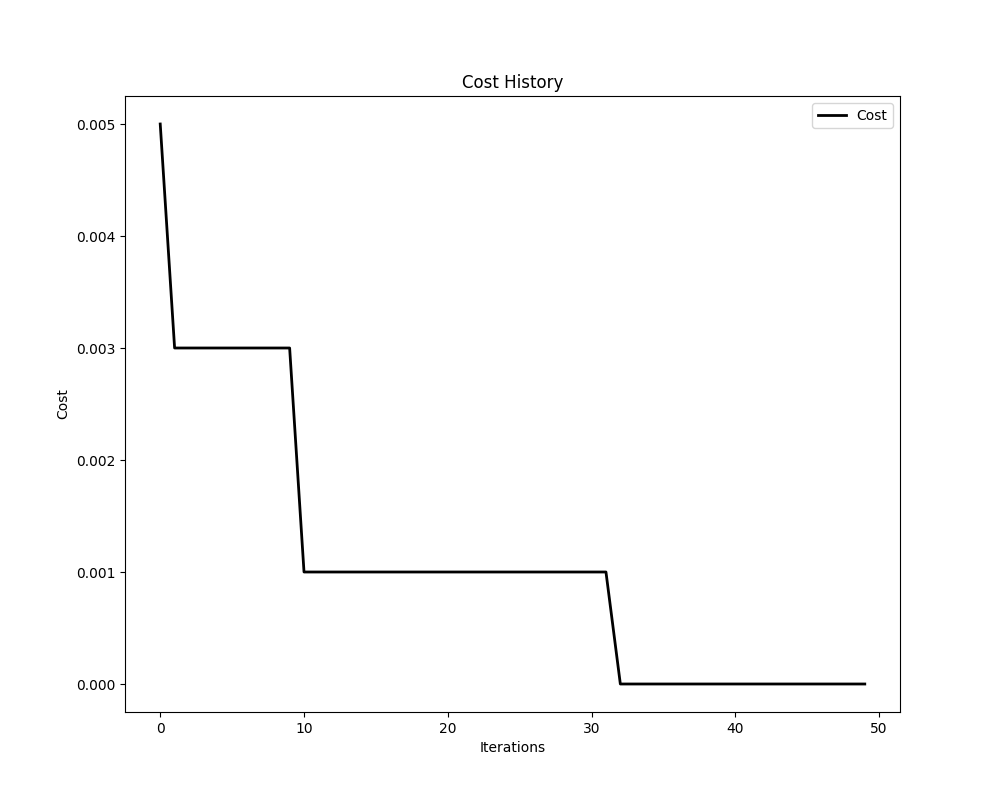
\includegraphics[width=0.9\textwidth]{img/opti/costHistoryGini.png}
                \caption{Cost history of the Gini coefficient}
        \end{figure}

        \subsubsection{Statistical analysis}
        
            Our null hypothesis H0 is that our two samples (two sets of optimized parameters obtained by the same PSO on two different runs) have the same distribution. We will use an $\alpha$ value of 0.05 to test the hypothesis. Thus if we reject H0, i.e. the resulting p-value is < $\alpha$, our two PSOs have different distributions, otherwise, if the p-value is $> \alpha$, our two PSOs have identical distributions.

            We show in the following table (which is symmetrical of course) the p-values for each pair of two runs obtained by the \texttt{ranksums} function of the \texttt{scipy} library. All p-values are above our threshold of 0.05, i.e. all of our optimized parameters come from the same algorithm/distribution with a confidence level of 5\%.

\begin{table}[H]
    \centering
    \begin{tabular}{|c|c|c|c|c|c|c|c|c|c|c|}
        \hline
        \textbf{\#}& \textbf{1}& \textbf{2}& \textbf{3}& \textbf{4}& \textbf{5}& \textbf{6}& \textbf{7}& \textbf{8}& \textbf{9}& \textbf{10}\\ \hline
        \textbf{1}  & 1.0 & 1.0 & 1.0 & 0.337 & 0.631 & 0.749 & 0.631 & 0.749 & 0.423 & 0.749\\ \hline
        \textbf{2}  & 1.0 & 1.0 & 0.423 & 0.262 & 0.262 & 0.337 & 0.631 & 0.423 & 0.15 & 0.423\\ \hline
        \textbf{3}  & 1.0 & 0.423 & 1.0 & 0.631 & 1.0 & 0.749 & 0.631 & 0.631 & 0.749 & 0.873\\ \hline
        \textbf{4}  & 0.337 & 0.262 & 0.631 & 1.0 & 0.2 & 0.522 & 0.749 & 0.2 & 0.2 & 0.2\\ \hline
        \textbf{5}  & 0.631 & 0.262 & 1.0 & 0.2 & 1.0 & 0.522 & 0.423 & 0.873 & 0.631 & 0.631\\ \hline
        \textbf{6}  & 0.749 & 0.337 & 0.749 & 0.522 & 0.522 & 1.0 & 0.337 & 0.522 & 0.873 & 0.423\\ \hline
        \textbf{7}  & 0.631 & 0.631 & 0.631 & 0.749 & 0.423 & 0.337 & 1.0 & 0.631 & 0.262 & 0.522\\ \hline
        \textbf{8}  & 0.749 & 0.423 & 0.631 & 0.2 & 0.873 & 0.522 & 0.631 & 1.0 & 0.423 & 0.631\\ \hline
        \textbf{9}  & 0.423 & 0.15 & 0.749 & 0.2 & 0.631 & 0.873 & 0.262 & 0.423 & 1.0 & 0.522\\ \hline
        \textbf{10}  & 0.749 & 0.423 & 0.873 & 0.2 & 0.631 & 0.423 & 0.522 & 0.631 & 0.522 & 1.0\\ \hline
    \end{tabular}
\end{table}
            
        

    \subsection{GDP}

        Naturally, we want to maximize the GDP of a State. The following results were obtained.
    
        \subsubsection{Optimized parameters}

            \begin{table}[H]
            \centering
            \begin{tabular}{|c|c|c|c|c|c|c|c|}
                \hline
                \textbf{\#} & \textbf{GDP}  & \textbf{VAT} & \textbf{Levy} & \textbf{Tariff} & \textbf{Wealth} & \textbf{Unemployment} & \textbf{Black} \\ \hline
                \textbf{1} & 36 739 & 0.043 & 0.729 & 0.376 & 0.769 & 0.309 & 0.036 \\ \hline
                \textbf{2} & 37 152 & 0.054 & 0.651 & 0.272 & 0.988 & 0.175 & 0.018 \\ \hline
                \textbf{3} & 36 749 & 0.059 & 0.945 & 0.528 & 0.021 & 0.337 & 0.034 \\ \hline
                \textbf{4} & 37 691 & 0.005 & 0.994 & 0.675 & 0.66 & 0.268 & 0.052 \\ \hline
                \textbf{5} & 36 334 & 0.0 & 0.846 & 0.537 & 0.833 & 0.387 & 0.014 \\ \hline
                \textbf{6} & 36 453 & 0.001 & 0.819 & 0.443 & 0.209 & 0.077 & 0.081 \\ \hline
                \textbf{7} & 36 703 & 0.043 & 0.91 & 0.505 & 0.285 & 0.13 & 0.006 \\ \hline
                \textbf{8} & 35 130 & 0.025 & 0.47 & 0.525 & 0.51 & 0.285 & 0.082 \\ \hline
                \textbf{9} & 35 556 & 0.198 & 0.944 & 0.37 & 0.957 & 0.423 & 0.028 \\ \hline
                \textbf{10} & 36 339 & 0.109 & 0.924 & 0.519 & 0.426 & 0.096 & 0.047 \\ \hline
            \end{tabular}
            \end{table}

            We can see some interesting patterns in the table. Indeed, we see that the VAT rates are very close to one another, the same goes for the black economy share. This actually fits our state-of-the-art and our experiments. Indeed, if we see, for instance, in \nameref{exp:black}, we had noticed that, as the black economy share grows, the GDP decreases. Therefore, reducing black economy at such low levels drastically increases the GDP.
            On the other side, we see no real pattern for the other parameters, i.e. they do not significantly influence the GDP.

            We can also see in the following plot the decrease of the GDP across iterations (cost history). PSO will minimize the opposite of the GDP (thus maximizing the GDP), that is why the costs are negative, and we want them to be as low as possible.

            \begin{figure}[H]
                \centering
                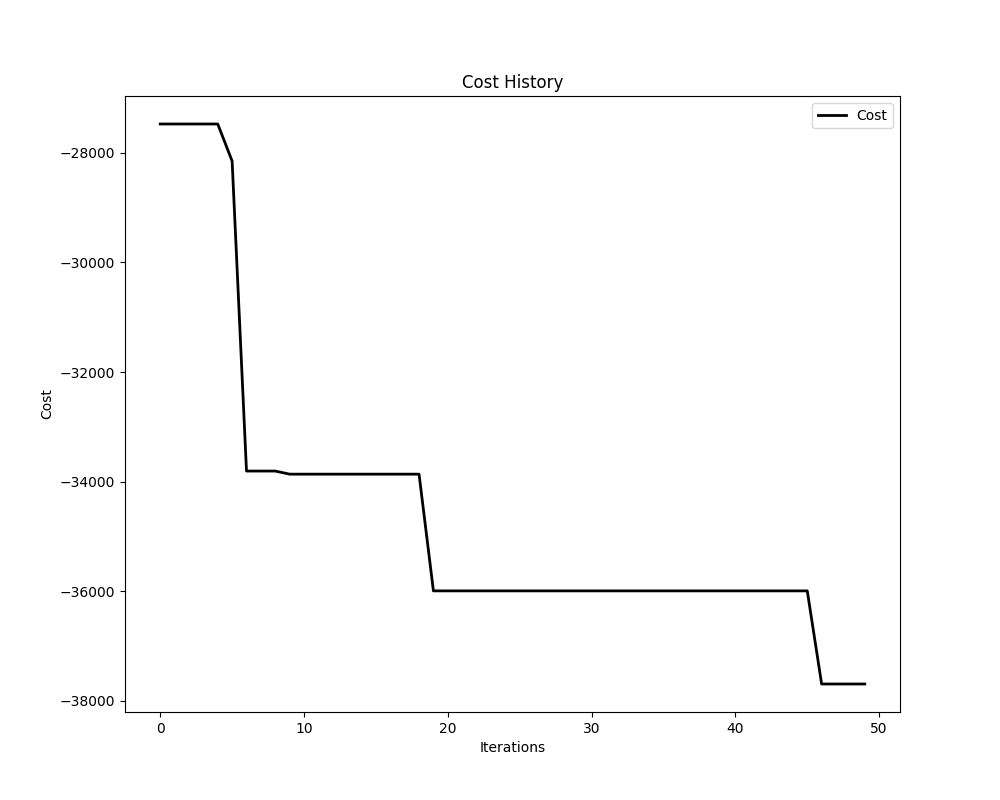
\includegraphics[width=0.9\textwidth]{img/opti/costHistoryGDP.png}
                \caption{Cost history of the GDP}
            \end{figure}

        \subsubsection{Statistical analysis}

        Again, our null hypothesis H0 is that our two samples (two sets of optimized parameters obtained by the same PSO on two different runs) have the same distribution. We will use an $\alpha$ value of 0.05 to test the hypothesis. 

        We show in the following table the p-values for each pair of two runs obtained by the \texttt{ranksums} function of the \texttt{scipy} library. All p-values are above our threshold of 0.05, i.e. all of our optimized parameters come from the same algorithm/distribution with a confidence level of 5\%.

\begin{table}[H]
\centering
\begin{tabular}{|c|c|c|c|c|c|c|c|c|c|c|}
    \hline
    \textbf{\#}& \textbf{1}& \textbf{2}& \textbf{3}& \textbf{4}& \textbf{5}& \textbf{6}& \textbf{7}& \textbf{8}& \textbf{9}& \textbf{10}\\ \hline
    \textbf{1}  & 1.0 & 0.749 & 0.631 & 1.0 & 0.749 & 0.749 & 0.689 & 0.749 & 0.631 & 0.749\\ \hline
    \textbf{2}  & 0.749 & 1.0 & 0.873 & 0.749 & 1.0 & 0.749 & 0.749 & 0.873 & 0.522 & 1.0\\ \hline
    \textbf{3}  & 0.631 & 0.873 & 1.0 & 0.631 & 0.873 & 1.0 & 0.873 & 0.873 & 0.423 & 0.631\\ \hline
    \textbf{4}  & 1.0 & 0.749 & 0.631 & 1.0 & 0.873 & 0.522 & 0.631 & 0.631 & 0.873 & 0.749\\ \hline
    \textbf{5}  & 0.749 & 1.0 & 0.873 & 0.873 & 1.0 & 0.522 & 0.749 & 0.631 & 0.631 & 1.0\\ \hline
    \textbf{6}  & 0.749 & 0.749 & 1.0 & 0.522 & 0.522 & 1.0 & 0.749 & 0.423 & 0.337 & 0.522\\ \hline
    \textbf{7}  & 0.689 & 0.749 & 0.873 & 0.631 & 0.749 & 0.749 & 1.0 & 0.689 & 0.337 & 0.631\\ \hline
    \textbf{8}  & 0.749 & 0.873 & 0.873 & 0.631 & 0.631 & 0.423 & 0.689 & 1.0 & 0.631 & 0.873\\ \hline
    \textbf{9}  & 0.631 & 0.522 & 0.423 & 0.873 & 0.631 & 0.337 & 0.337 & 0.631 & 1.0 & 0.631\\ \hline
    \textbf{10}  & 0.749 & 1.0 & 0.631 & 0.749 & 1.0 & 0.522 & 0.631 & 0.873 & 0.631 & 1.0\\ \hline
\end{tabular}
\end{table}

    \subsection{Number of transactions}

        Naturally, we want to maximize the number of transactions in a State. The following results were obtained.
    
        \subsubsection{Optimized parameters}
            
            \begin{table}[H]
            \centering
            \begin{tabular}{|c|c|c|c|c|c|c|c|}
                \hline
                \textbf{\#} & \textbf{Nb transactions}  & \textbf{VAT} & \textbf{Levy} & \textbf{Tariff} & \textbf{Wealth} & \textbf{Unemployment} & \textbf{Black} \\ \hline
                \textbf{1} & 739 & 0.456 & 0.824 & 0.487 & 0.556 & 0.021 & 0.954 \\ \hline
                \textbf{2} & 788 & 0.741 & 0.871 & 0.18 & 0.462 & 0.063 & 0.996 \\ \hline
                \textbf{3} & 753 & 0.708 & 0.906 & 0.939 & 0.884 & 0.041 & 0.993 \\ \hline
                \textbf{4} & 737 & 0.419 & 0.691 & 0.137 & 0.551 & 0.005 & 0.826 \\ \hline
                \textbf{5} & 726 & 0.091 & 0.924 & 0.904 & 0.175 & 0.044 & 0.714 \\ \hline
                \textbf{6} & 752 & 0.412 & 0.759 & 0.554 & 0.671 & 0.004 & 0.917 \\ \hline
                \textbf{7} & 747 & 0.608 & 0.974 & 0.588 & 0.743 & 0.005 & 0.957 \\ \hline
                \textbf{8} & 725 & 0.306 & 0.682 & 0.55 & 0.794 & 0.062 & 0.962 \\ \hline
                \textbf{9} & 740 & 0.963 & 0.858 & 0.323 & 0.472 & 0.018 & 0.994 \\ \hline
                \textbf{10} & 746 & 0.672 & 0.479 & 0.073 & 0.809 & 0.001 & 0.954 \\ \hline
            \end{tabular}
            \end{table}

            We can see two patterns emerging. First, for the number of transactions to be high, we need a very small unemployment rate as we can see on the table (i.e. this is the `common denominator' of all these optimizations). This makes sense, because more unemployment means more non-producers, therefore less products on the market to buy and less transactions. This fits our \nameref{exp:unemployment} where we saw a linear correlation between the unemployment rate and the number of transactions.

            Secondly, we can see that, generally but not always, the black economy share is very high. This is due to the fact that a black transaction is still counted towards the total number of transactions, however no due taxes are paid. This is quite surprising as it is not exactly what we had seen in \nameref{exp:black} where we saw no real correlation between the black economy share and the number of transactions. This is probably due to the fact that now, we have a very high levy tax compared to before where the default configuration set it at 0.1.

            We can also see in the following plot the decrease of the number of transactions across iterations (cost history). PSO will minimize the opposite of the number of transactions (thus maximizing the number of transactions), that is why the costs are negative, and we want them to be as low as possible.

            \begin{figure}[H]
                \centering
                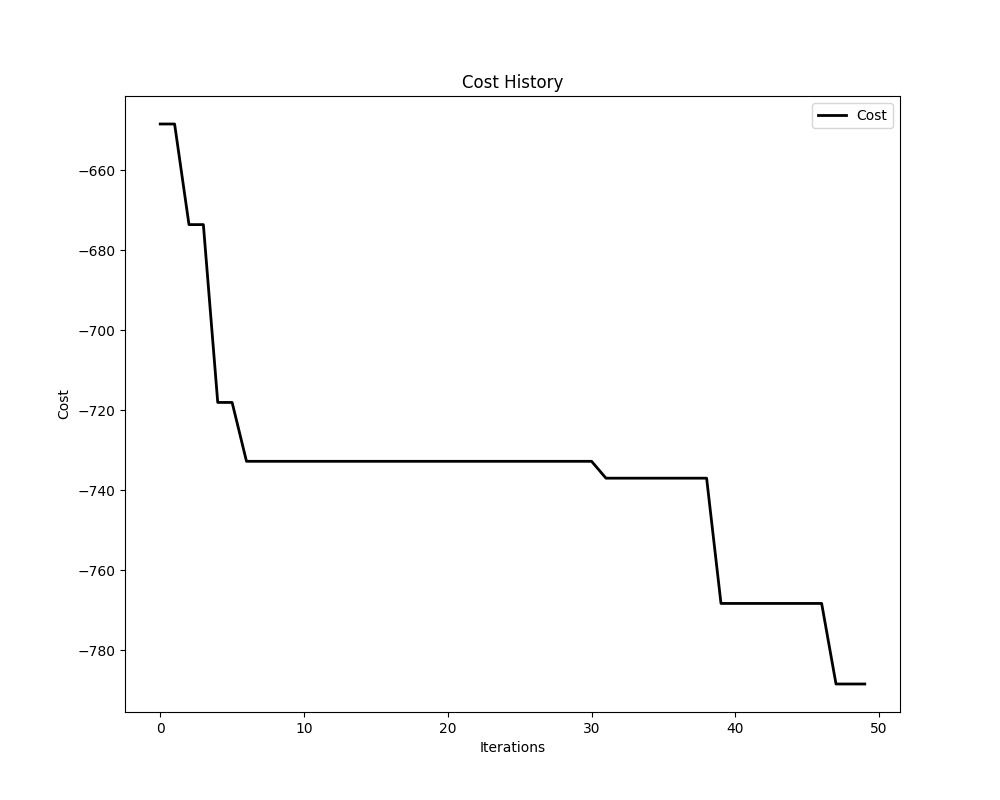
\includegraphics[width=0.9\textwidth]{img/opti/costHistoryNbTransactions.png}
                \caption{Cost history of the number of transactions}
            \end{figure}


        \subsubsection{Statistical analysis}

        Again, our null hypothesis H0 is that our two samples (two sets of optimized parameters obtained by the same PSO on two different runs) have the same distribution. We will use an $\alpha$ value of 0.05 to test the hypothesis. 

        We show in the following table the p-values for each pair of two runs obtained by the \texttt{ranksums} function of the \texttt{scipy} library. All p-values are above our threshold of 0.05, i.e. all of our optimized parameters come from the same algorithm/distribution with a confidence level of 5\%.

\begin{table}[H]
\centering
\begin{tabular}{|c|c|c|c|c|c|c|c|c|c|c|}
    \hline
    \textbf{\#}& \textbf{1}& \textbf{2}& \textbf{3}& \textbf{4}& \textbf{5}& \textbf{6}& \textbf{7}& \textbf{8}& \textbf{9}& \textbf{10}\\ \hline
    \textbf{1}  & 1.0 & 0.873 & 0.2 & 0.522 & 0.873 & 0.873 & 0.337 & 0.873 & 0.749 & 0.749\\ \hline
    \textbf{2}  & 0.873 & 1.0 & 0.423 & 0.423 & 0.631 & 0.873 & 0.749 & 0.873 & 0.873 & 0.749\\ \hline
    \textbf{3}  & 0.2 & 0.423 & 1.0 & 0.055 & 0.337 & 0.15 & 0.522 & 0.262 & 0.631 & 0.2\\ \hline
    \textbf{4}  & 0.522 & 0.423 & 0.055 & 1.0 & 0.631 & 0.631 & 0.2 & 0.631 & 0.337 & 0.873\\ \hline
    \textbf{5}  & 0.873 & 0.631 & 0.337 & 0.631 & 1.0 & 1.0 & 0.522 & 0.749 & 0.522 & 0.873\\ \hline
    \textbf{6}  & 0.873 & 0.873 & 0.15 & 0.631 & 1.0 & 1.0 & 0.423 & 0.873 & 0.631 & 1.0\\ \hline
    \textbf{7}  & 0.337 & 0.749 & 0.522 & 0.2 & 0.522 & 0.423 & 1.0 & 0.631 & 1.0 & 0.423\\ \hline
    \textbf{8}  & 0.873 & 0.873 & 0.262 & 0.631 & 0.749 & 0.873 & 0.631 & 1.0 & 0.631 & 0.749\\ \hline
    \textbf{9}  & 0.749 & 0.873 & 0.631 & 0.337 & 0.522 & 0.631 & 1.0 & 0.631 & 1.0 & 0.522\\ \hline
    \textbf{10}  & 0.749 & 0.749 & 0.2 & 0.873 & 0.873 & 1.0 & 0.423 & 0.749 & 0.522 & 1.0\\ \hline
\end{tabular}
\end{table}

\chapter{Conclusion}

Throughout this thesis, we have been exploring the role of many key parameters that are part of most economical systems around the world. For this, we have simulated an economical system (the World) by generating many homogeneous and independent agents belonging to different States with different parameters. All these agents interact with each other according to certain rules edicted by their States. 

We have seen the State-of-the-art research regarding both economics and computer science in order to be better equipped for the simulation, the experiments and the optimization. This allowed us to have a base for future comparisons, and see whether or not our results fitted the actual reality.

By letting these agents interact with one another throughout ticks (representing time passing by), we were able to see emerging patterns on certain metrics such as the Gini coefficient or the number of transactions. By modifying some initial parameters, we could influence the final metrics, therefore allowing us to understand the role of each parameter as we have seen in the \nameref{chap:Experiments} chapter. We have also compared this experiments with State-of-the-art research happening in both the computer science and economics fields. Most experiments fitted the reality depicted by these research, however, a few did not, due to the complexity of the task.

To go even further, we tried to optimize some key parameters of the State in order to minimize or maximize some metrics. This was done through the use of Particle Swarm Optimization, a population-based method, which let us optimize continuous variables method. This was done to confirm the role of each parameter and how States could improve these metrics. We have seen that these results fitted the ones we have in our experiments as well as the ones in the State-of-the-art.

As we have previously stated, this computer simulation is far from being perfect or close to reality. We tried to focus ourselves on the big picture and the essential parts of an economical system at the cost of precision. There is still a lot of room for improvement. Indeed, in future works, we could improve this by taking into account many new parameters such as the quality of a product or its carbon footprint,  create luxurious products, have multiple clusters, different types of agreements between States, analyze imports and exports, use multi-objective optimization to optimize multiple metrics at the same time, create an Graphic User Interface (GUI) for easier use, ...

\newpage

\chapter{References}
\printbibliography[heading=none]

\end{document}
